%!TEX root = ../dissertation.tex

\chapter{Evaluation}
\label{chapter:evaluation}
The present chapter describes the evaluation methodology as well as the experiments performed to determine
if a cloud-based or a fog-based approach is more adequate to deploy \gls{RFID} applications in a
smart warehouse. The evaluation process will focus on establish if the approaches are
able to met the low-latency and data storage performance requirements described in \ref{table:eval_requirements}.\\

Our main goal is to obtain basic statistical values - e.g. average - that allow us to decide which
approach is more suitable to fulfill the expected requirements. Furthermore, according to the obtained
results we intend to specify which approach is more adequate to deploy an \gls{IoT} application regarding
its domain.

% 2. Present the evaluation methodology for both cases
\section{Evaluation Methodology}
\label{sec:eval_methodology}
In order to determine which approach is more adequate to meet the latency and data storage scalability
requirements, we propose the following methodologies to perform the evaluation:

% Evaluation Methodologies : Latency
\subsection{Latency Interaction}
\label{sub:eval_methodology_latency}
The response time between an event that occurs in the smart warehouse and the corresponding action
that is triggered in the physical space will be evaluated according the methodology proposed in
Figure~\ref{fig:eval_latency_methodology}.\\

% Latency Interaction Evaluation Methodology Figure
\begin{figure}[ht!]
  \centering
  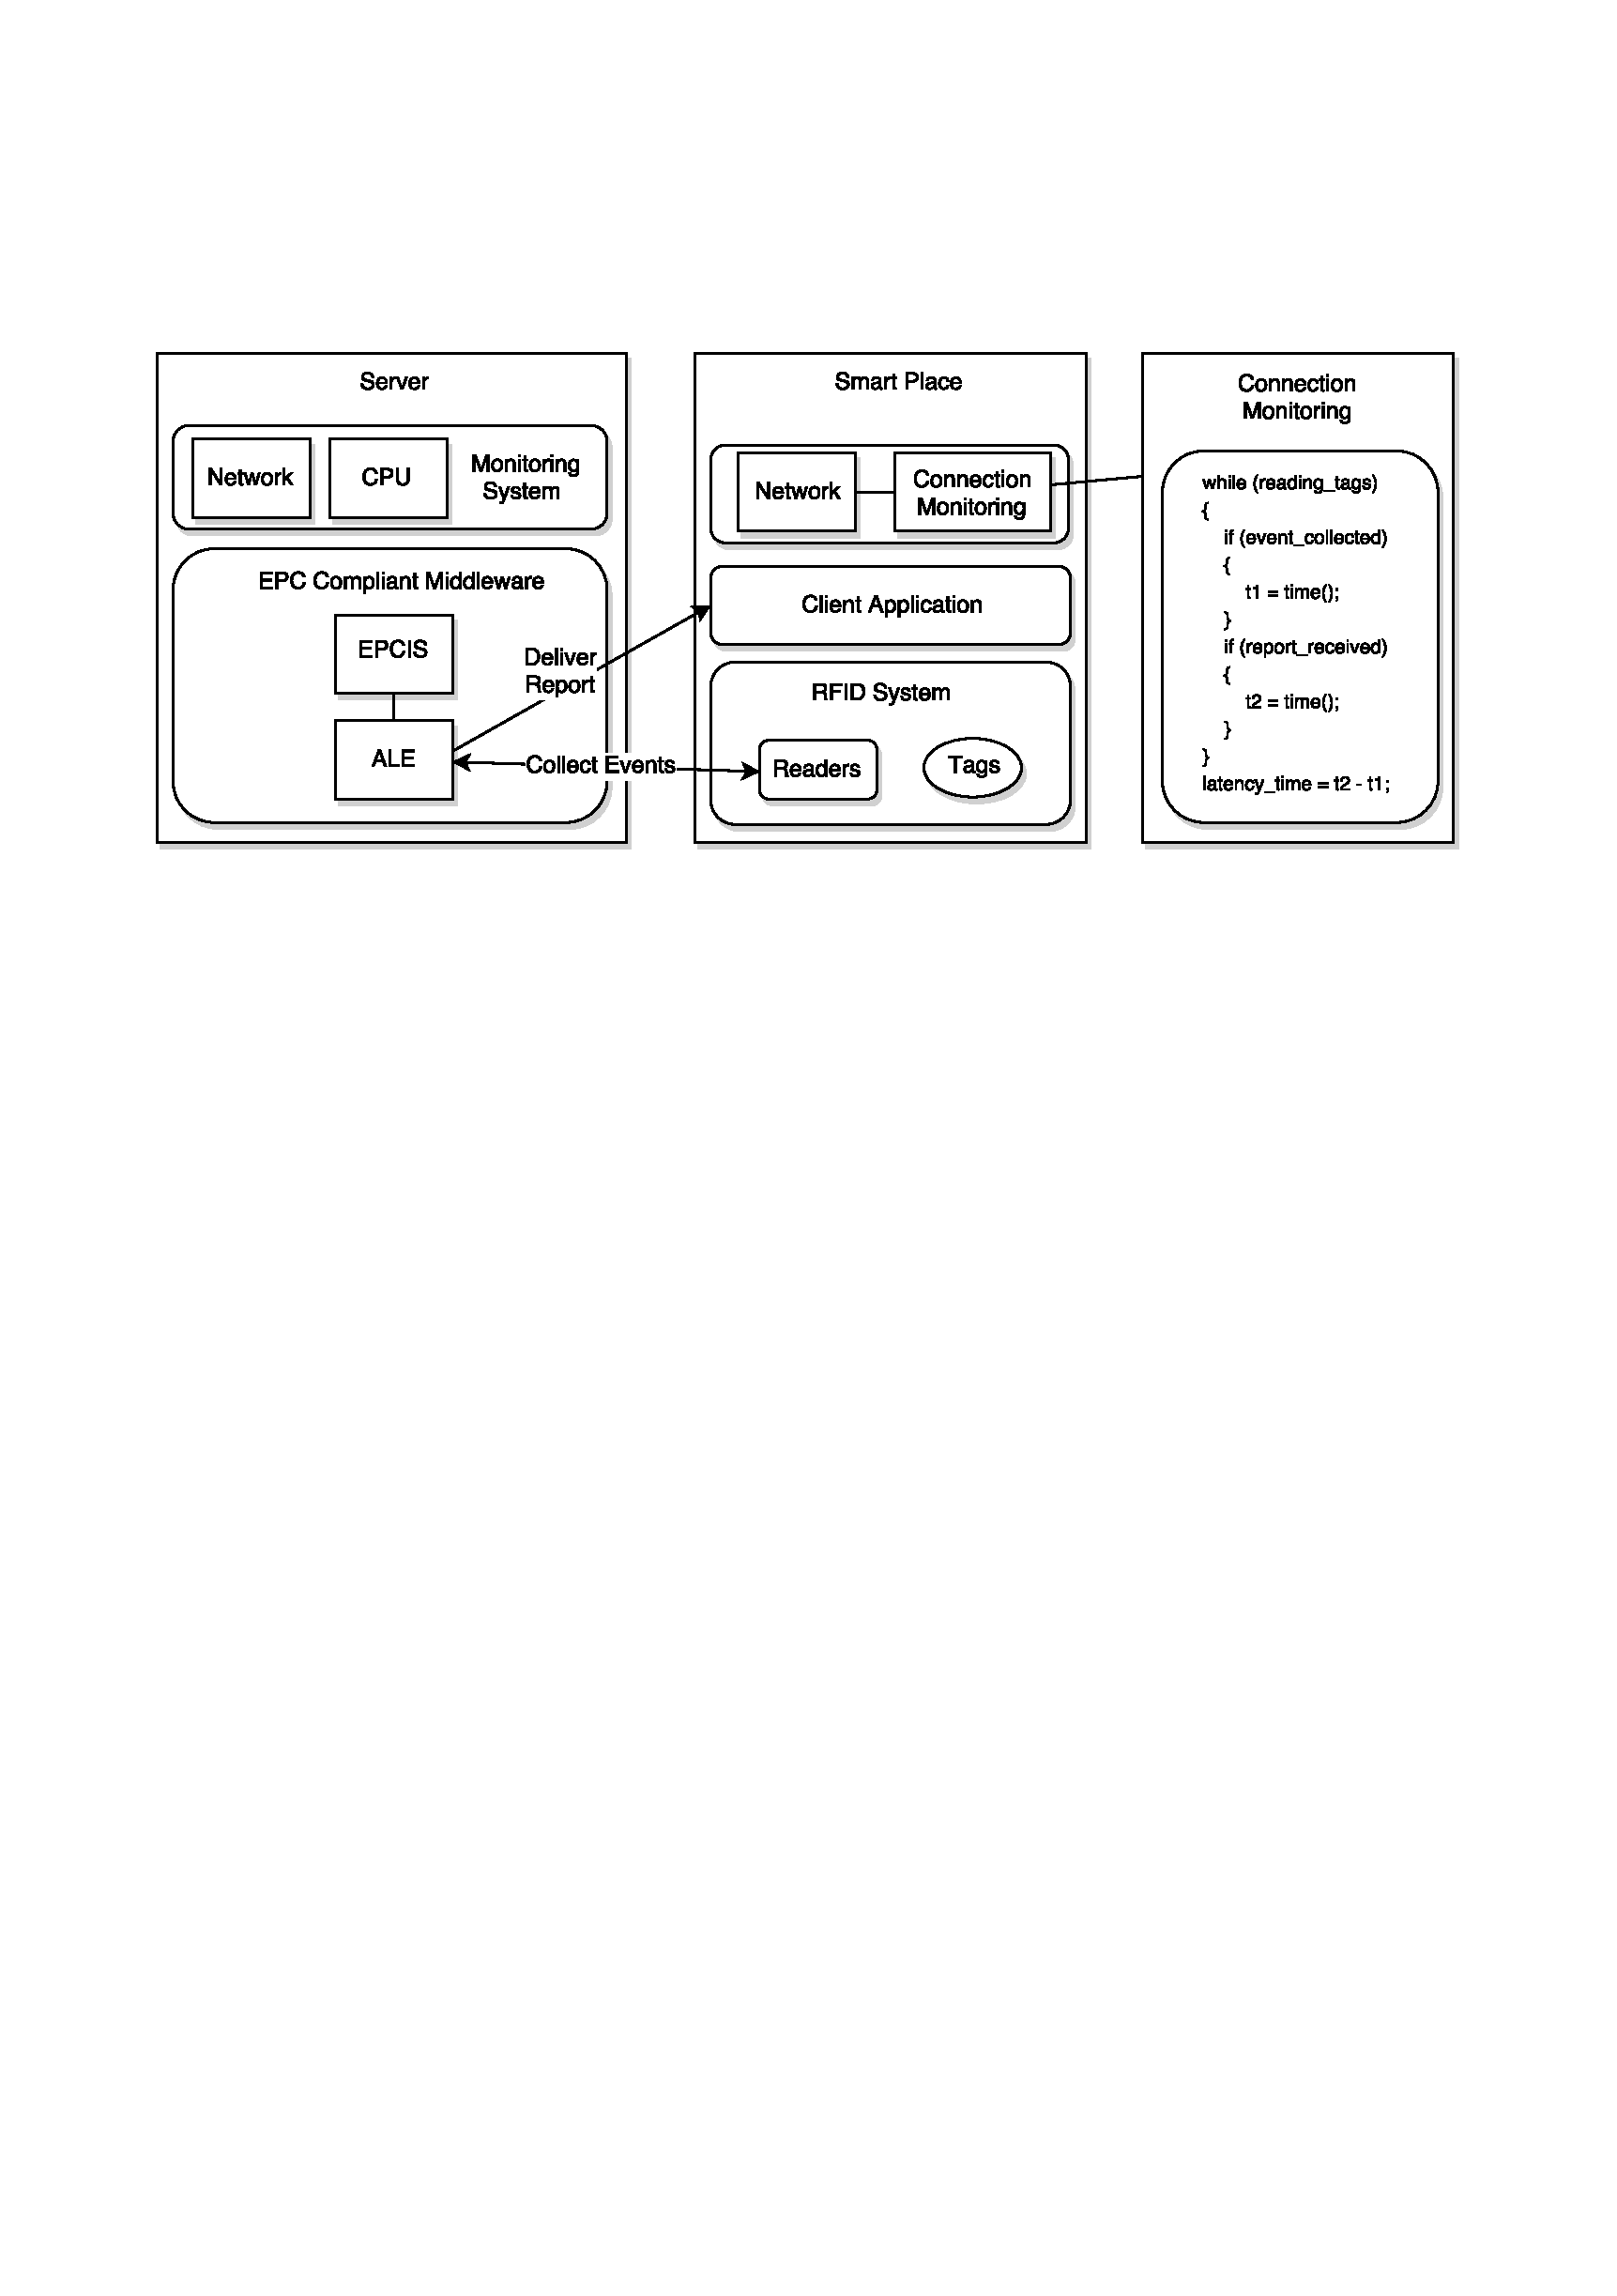
\includegraphics[width=.9\textwidth]{./images/eval_latency_methodology}
  \caption[Latency evaluation methodology.]{Latency interaction evaluation methodology.}
  \label{fig:eval_latency_methodology}
\end{figure}

The \gls{ALE} module is responsible for collecting and processing the reader events and take the
correct decisions based on those events. In the Fosstrak implementation the collection and processing
of reader events is performed according to an \textit{Event Cycle} specification. The \textit{Event Cycle}
is a set of periodical cycles where the \gls{ALE} module collect the events from the readers. The data
about the \textit{Event Cycle} is delivered to the client application through a report. The information
in the report can be used to notify the client regarding an event in the smart warehouse or even to
trigger a new event in the warehouse such as open or close a door.\\

The smart warehouse is running a monitoring system that stores information about the incoming and outgoing
connections. The Fosstrak \gls{ALE} module can be configured to generate information to register
when a new event is processed and also when a new report is delivered to the client. Thus, with the
information provided by the monitoring system and the \gls{ALE} module it is possible to calculate
the latency request for an event that occurs in the warehouse.\\

With this methodology we intend to obtain information regarding how the communication time is spent
when an event is triggered in the warehouse for the approaches described in \ref{chapter:solution}.
In order to determine which approach is more adequate to deploy the application, we proposed the
following metrics:

% Metrics
\begin{itemize}
  \item \textit{Event Latency}: the time spent since an event is triggered in the warehouse until
  the client application receives the notification of the event.
  \item \textit{Upload Latency}: the time spent since that an event is triggered in the warehouse until
  the \gls{ALE} module receives the event.
  \item \textit{Tag Processing Latency}: the time spent since that the \gls{ALE} module receives an event
  notification until the \gls{RFID} tag is processed.
  \item \textit{Idle Processing Latency}: the time spent for the \gls{ALE} module where the collected
  tags already exists and no further action is required.
  \item \textit{Filtering \& Aggregation Latency}: the time spent for the \gls{ALE} where the
  collected tags are filtered and aggregated.
  \item \textit{Report Creation Latency}: the time spent for the \gls{ALE} module to create the
  \textit{Event Cycle} report for the current \textit{EventCycle}.
  \item \textit{Response Latency}: the time spent since that the \gls{ALE} module delivers the
  \textit{Event Cycle} report until the client receives it.
\end{itemize}

The analysis of these metrics will allow us to compare the performance of the fog-based and cloud-based
approaches and help to determine which one is more adequate to deploy the application in the warehouse.

% Evaluation Methodologies : Data Storage
\subsection{Data Storage Performance}
\label{sub:eval_methodology_data}
To evaluate the data storage performance for a \gls{RFID} application based on Fosstrak, the proposed
methodology consists in stress the \gls{EPCIS} Repository by simulating several users that are
concurrently sending events - through \gls{HTTP} requests - to the repository that is
running in the cloud, as illustrated in Figure~\ref{fig:eval_data_methodology}.

% Data Storage Evaluation Methodology Figure
\begin{figure}[ht!]
  \centering
  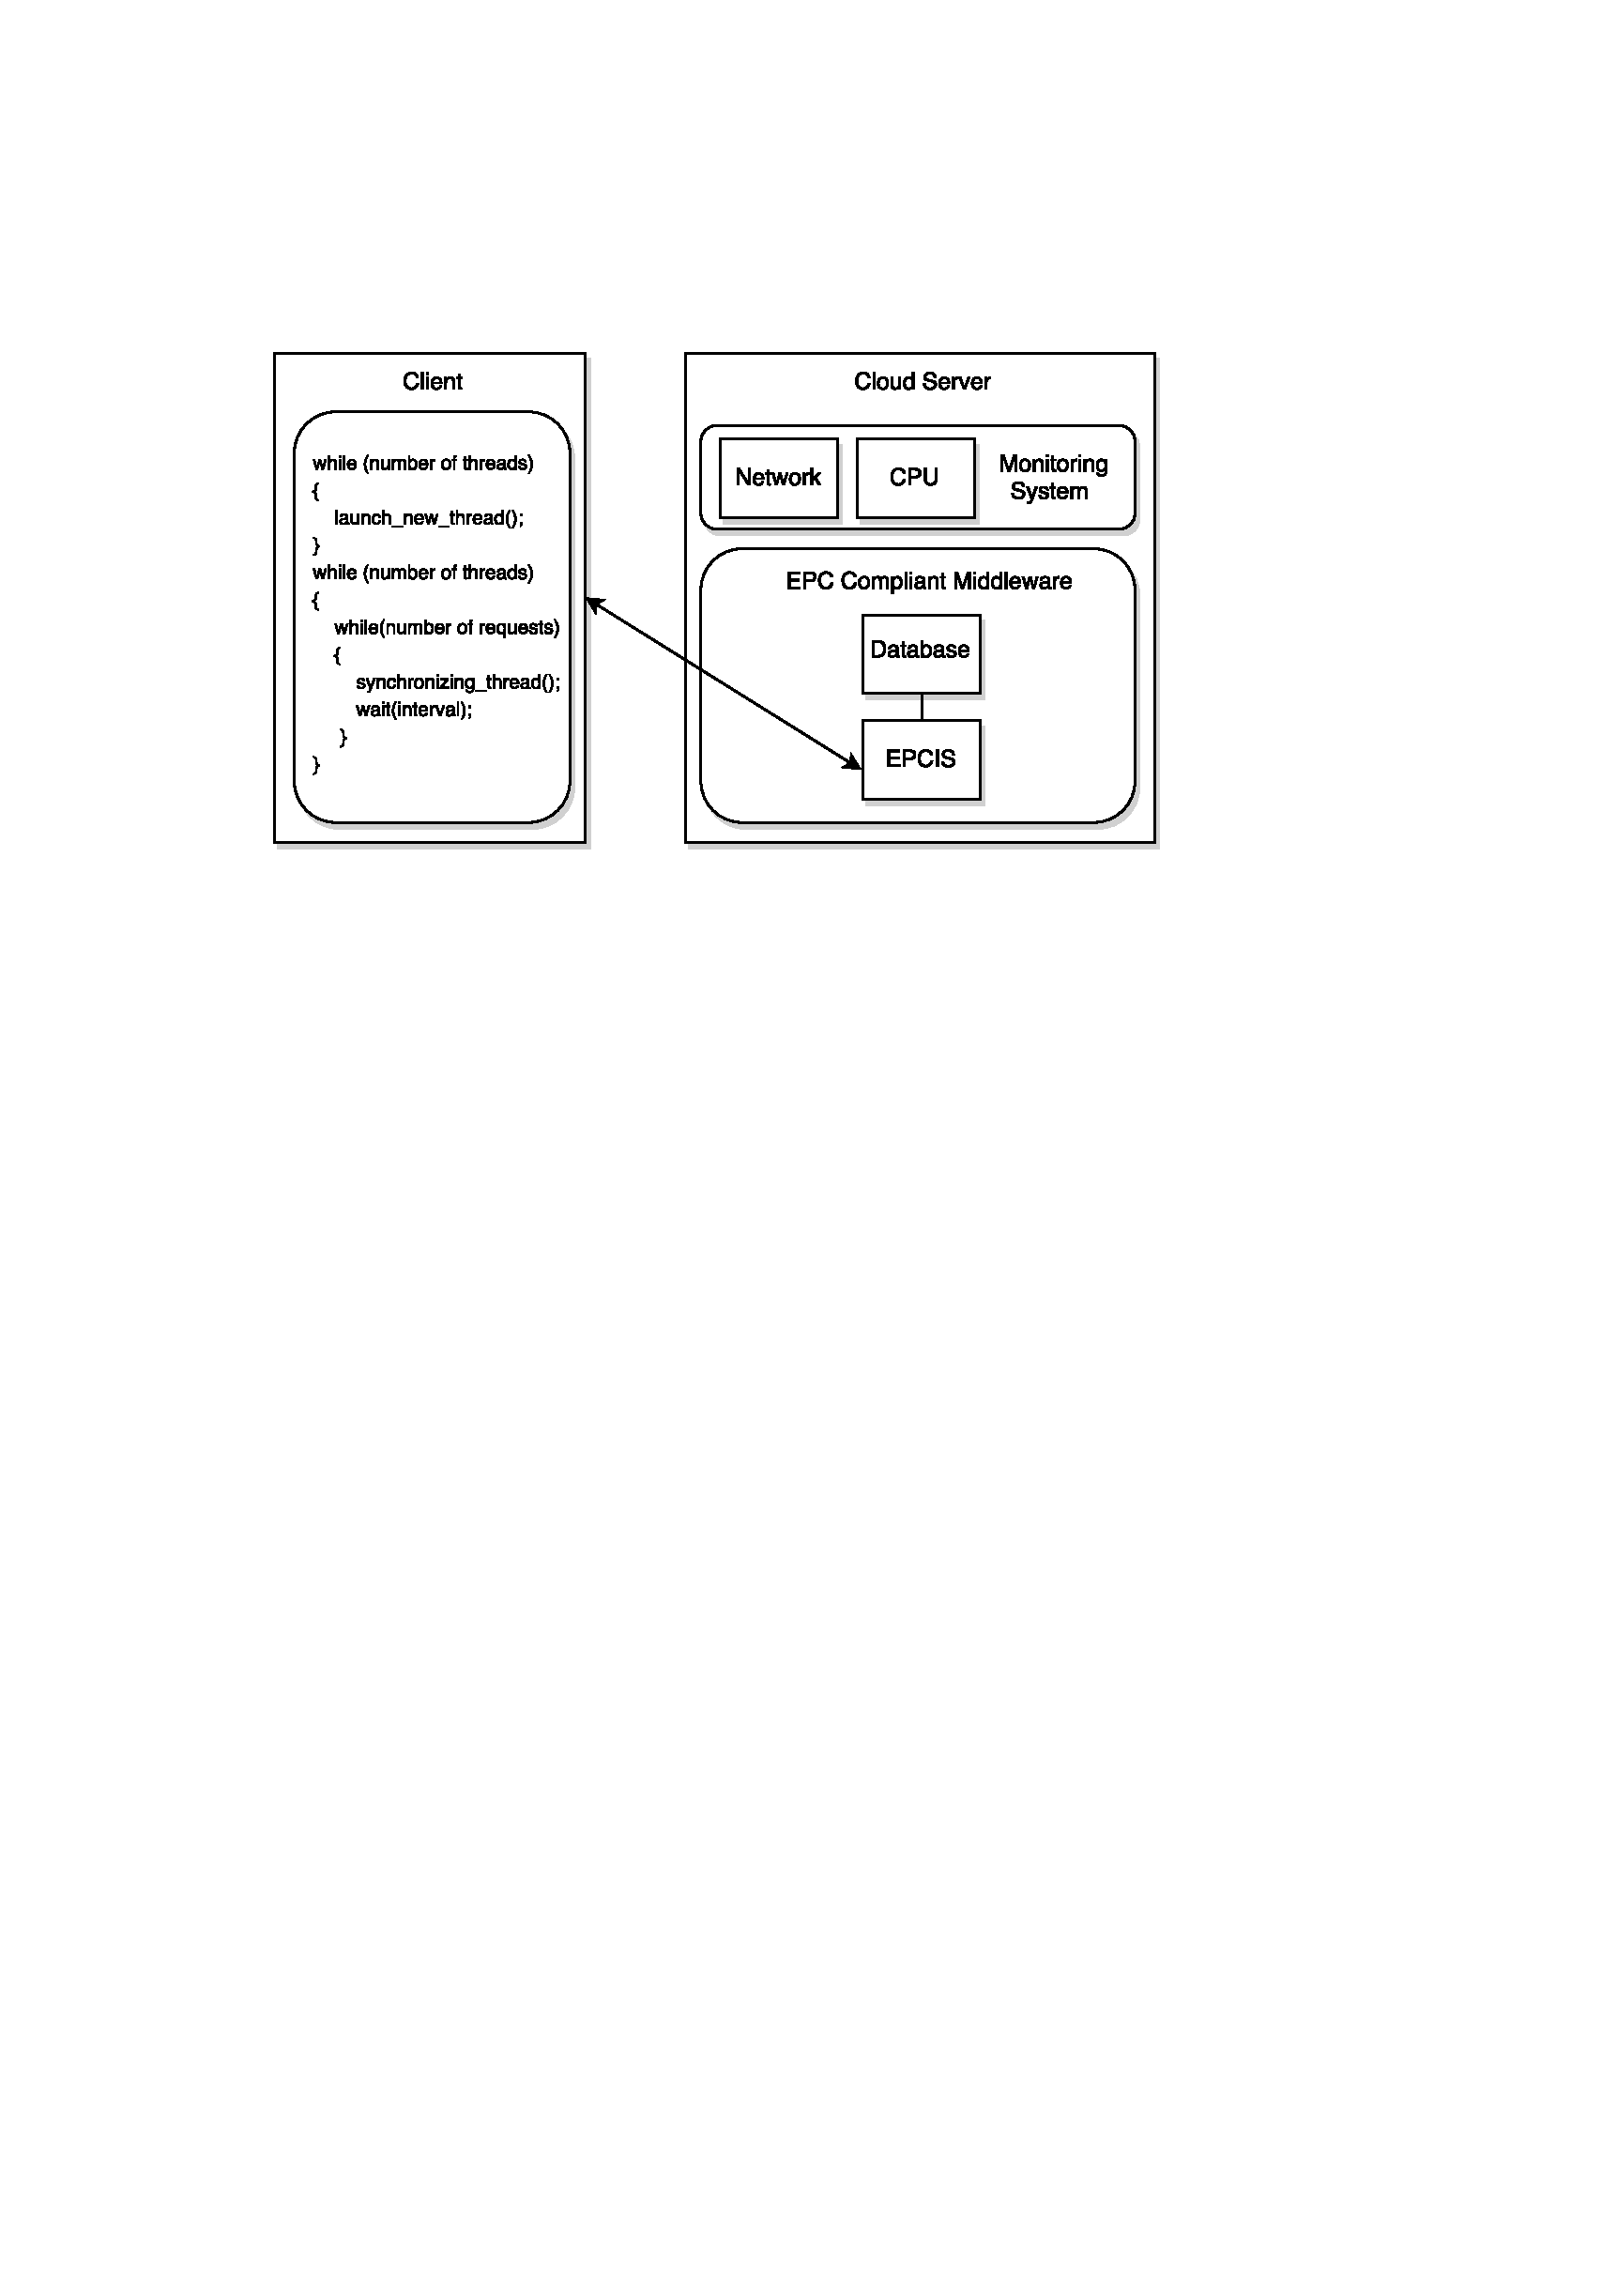
\includegraphics[width=.7\textwidth]{./images/eval_data_methodology}
  \caption[Data storage evaluation methodology.]{Data storage performance evaluation methodology.}
  \label{fig:eval_data_methodology}
\end{figure}

The cloud server is running a monitoring system that periodically stores data related to a set of
system metrics, such as \textit{CPU Utilization} and \textit{Network In}.\\

The analysis of those metrics allows to observe how the performance and behavior of the \gls{EPCIS}
module is affected regarding the amount of events that are generated in the smart warehouse.

% Evaluation Setup
\section{Evaluation Setup}
\label{sec:eval_setup}
To perform the evaluation experiments we chose \gls{AWS} as cloud provider. All the experiments were
conducted in \gls{AWS} \gls{EC2} instances running the Amazon Linux AMI operating system. The \glspl{VM}
presents a configuration with a 2.5 \textit{\gls{GHz}} single-core processor with 1 \textit{\gls{GB}} of
\gls{RAM}. In the fog-approach configuration, the experiments were conducted in a \gls{VM} with
a 2.6 \textit{\gls{GHz}} dual-core processor with 2 \textit{\gls{GB}} of \gls{RAM} and running
the \textit{Linux Ubuntu 14.04.2 LTS} operating system. Regarding the smart warehouse infrastructure,
the evaluation was performed through a \gls{ADSL} connection The Rifidi Emulator\footnote{\url{http://rifidi.org}}
used to emulate the \gls{RFID} readers is in version \textit{1.6.0}.\\

Regarding the software components, the application stack is composed of the \textit{Apache Tomcat 7.0.52.0}\footnote{\url{http://tomcat.apache.org/}}
with \textit{Java} version \textit{1.7.0} update \textit{79}. The \gls{RFID} middleware used was the Fosstrak
described in section \ref{sub:fosstrak}. The middleware stack is available at the Fosstrak's\footnote{\url{http://fosstrak.github.io/}}
source control system, and the versions were: a) \textit{\gls{FCServer}} version \textit{1.2.0}; b) \textit{Capture Application}
version \textit{0.1.1}; and c) \textit{\gls{EPCIS} Repository} version \textit{0.5.0}. Furthermore,
the \gls{EPCIS} Repository was connected to a \textit{MySQL server} version \textit{5.5}.\\

To monitoring the \glspl{VM} in the cloud and collect the system metrics from the instances, we use the
CloudWatch\footnote{\url{http://aws.amazon.com/cloudwatch/}} monitoring service provided by Amazon.

% Performed Experiments
\section{Experiments Performed}
\label{sec:eval_experiments}
The experiments performed in our evaluation were based on the scenario and data from the RFIDToys \cite{Correia:Thesis:2014}
Master Thesis.

\subsection{Latency Interaction}
\label{sub:eval_exp_latency}
To evaluate the latency interaction according the methodology proposed in Section~\ref{sub:eval_methodology_latency},
we use a scenario where a tagged robot was programmed to execute a given number of laps in the
warehouse plant where exists an automatic door that opens when one of the \gls{RFID} readers
that are placed in the plant detects that the robot is approaching. During the lap the robot stops during 5 seconds
in front of the door and then continues its lap. The door must be opened before the robot starts
to moving again.\\

The warehouse network connection was monitored with the \textit{tcpdump}\footnote{\url{http://www.tcpdump.org/}},
a command-line tool that allows to monitoring the packets that are being transmitted or received over
a network. Through the logs produced by this tool, we are able to determine how the connection time
is spent for the cloud-based approach and the fog-based approach.\\

Tho perform the simulation we defined two different specifications (\textit{ECspec}) for the
\textit{Event Cycles} of the \gls{ALE} module, \textit{Baseline Event Cycle} and
\textit{Half-period Event Cycle}. The configuration parameters for the \textit{ECspecs} are presented
in Table~\ref{table:ecspec_parameters}.

% ECspec parameters
\begin{table}[ht!]
 \begin{tabular}{|l|c|c|c|}
  \hline
  Event Cycle Specification & Period  & Duration & Repetitions \\ \hline
  Baseline Event Cycle      &  10s    & 9.5s     & 10          \\ \hline
  Half-period Event Cycle   &   5s    & 4.75s    & 20          \\ \hline
 \end{tabular}
 \caption[Event Cycle parameters.]{Event Cycle parameters.}
 \label{table:ecspec_parameters}
\end{table}

The evaluation of the event latency for the proposed approaches was performed in two steps. First,
we want to determine during a \textit{Event Cycle} how much time the \gls{ALE} is processing an event
and how much time the module is in an idle state. Furthermore, we want to determine how much time
takes each stage of the event processing pipeline. The event processing pipeline is divided in the
following stages: \textit{(i) the event data is uploaded}; \textit{(ii) event data is processed};
\textit{(iii) event data is filtered and aggregated}; \textit{(iv) the event cycle report is created};
and finally \textit{(v) the event cycle report is delivered to the client application}.

\subsubsection{Cloud-based warehouse latency}
\label{subs:eval_exp_latency_ecspec_fast}
Figure~\ref{fig:ecspecf_breakdown} summarizes the latency breakdown for an event that occurs in a cloud-based
smart warehouse. As in the previous experiment the \gls{ALE} module was configured with the
\textit{Baseline ECspec} and the \textit{Half-period ECspec}.\\

% Baseline ECspec event time breakdown
\begin{figure}[ht!]
  \centering
  % ECSpec Fast local breakdown figure
  \begin{subfigure}{.5\textwidth}
    \centering
    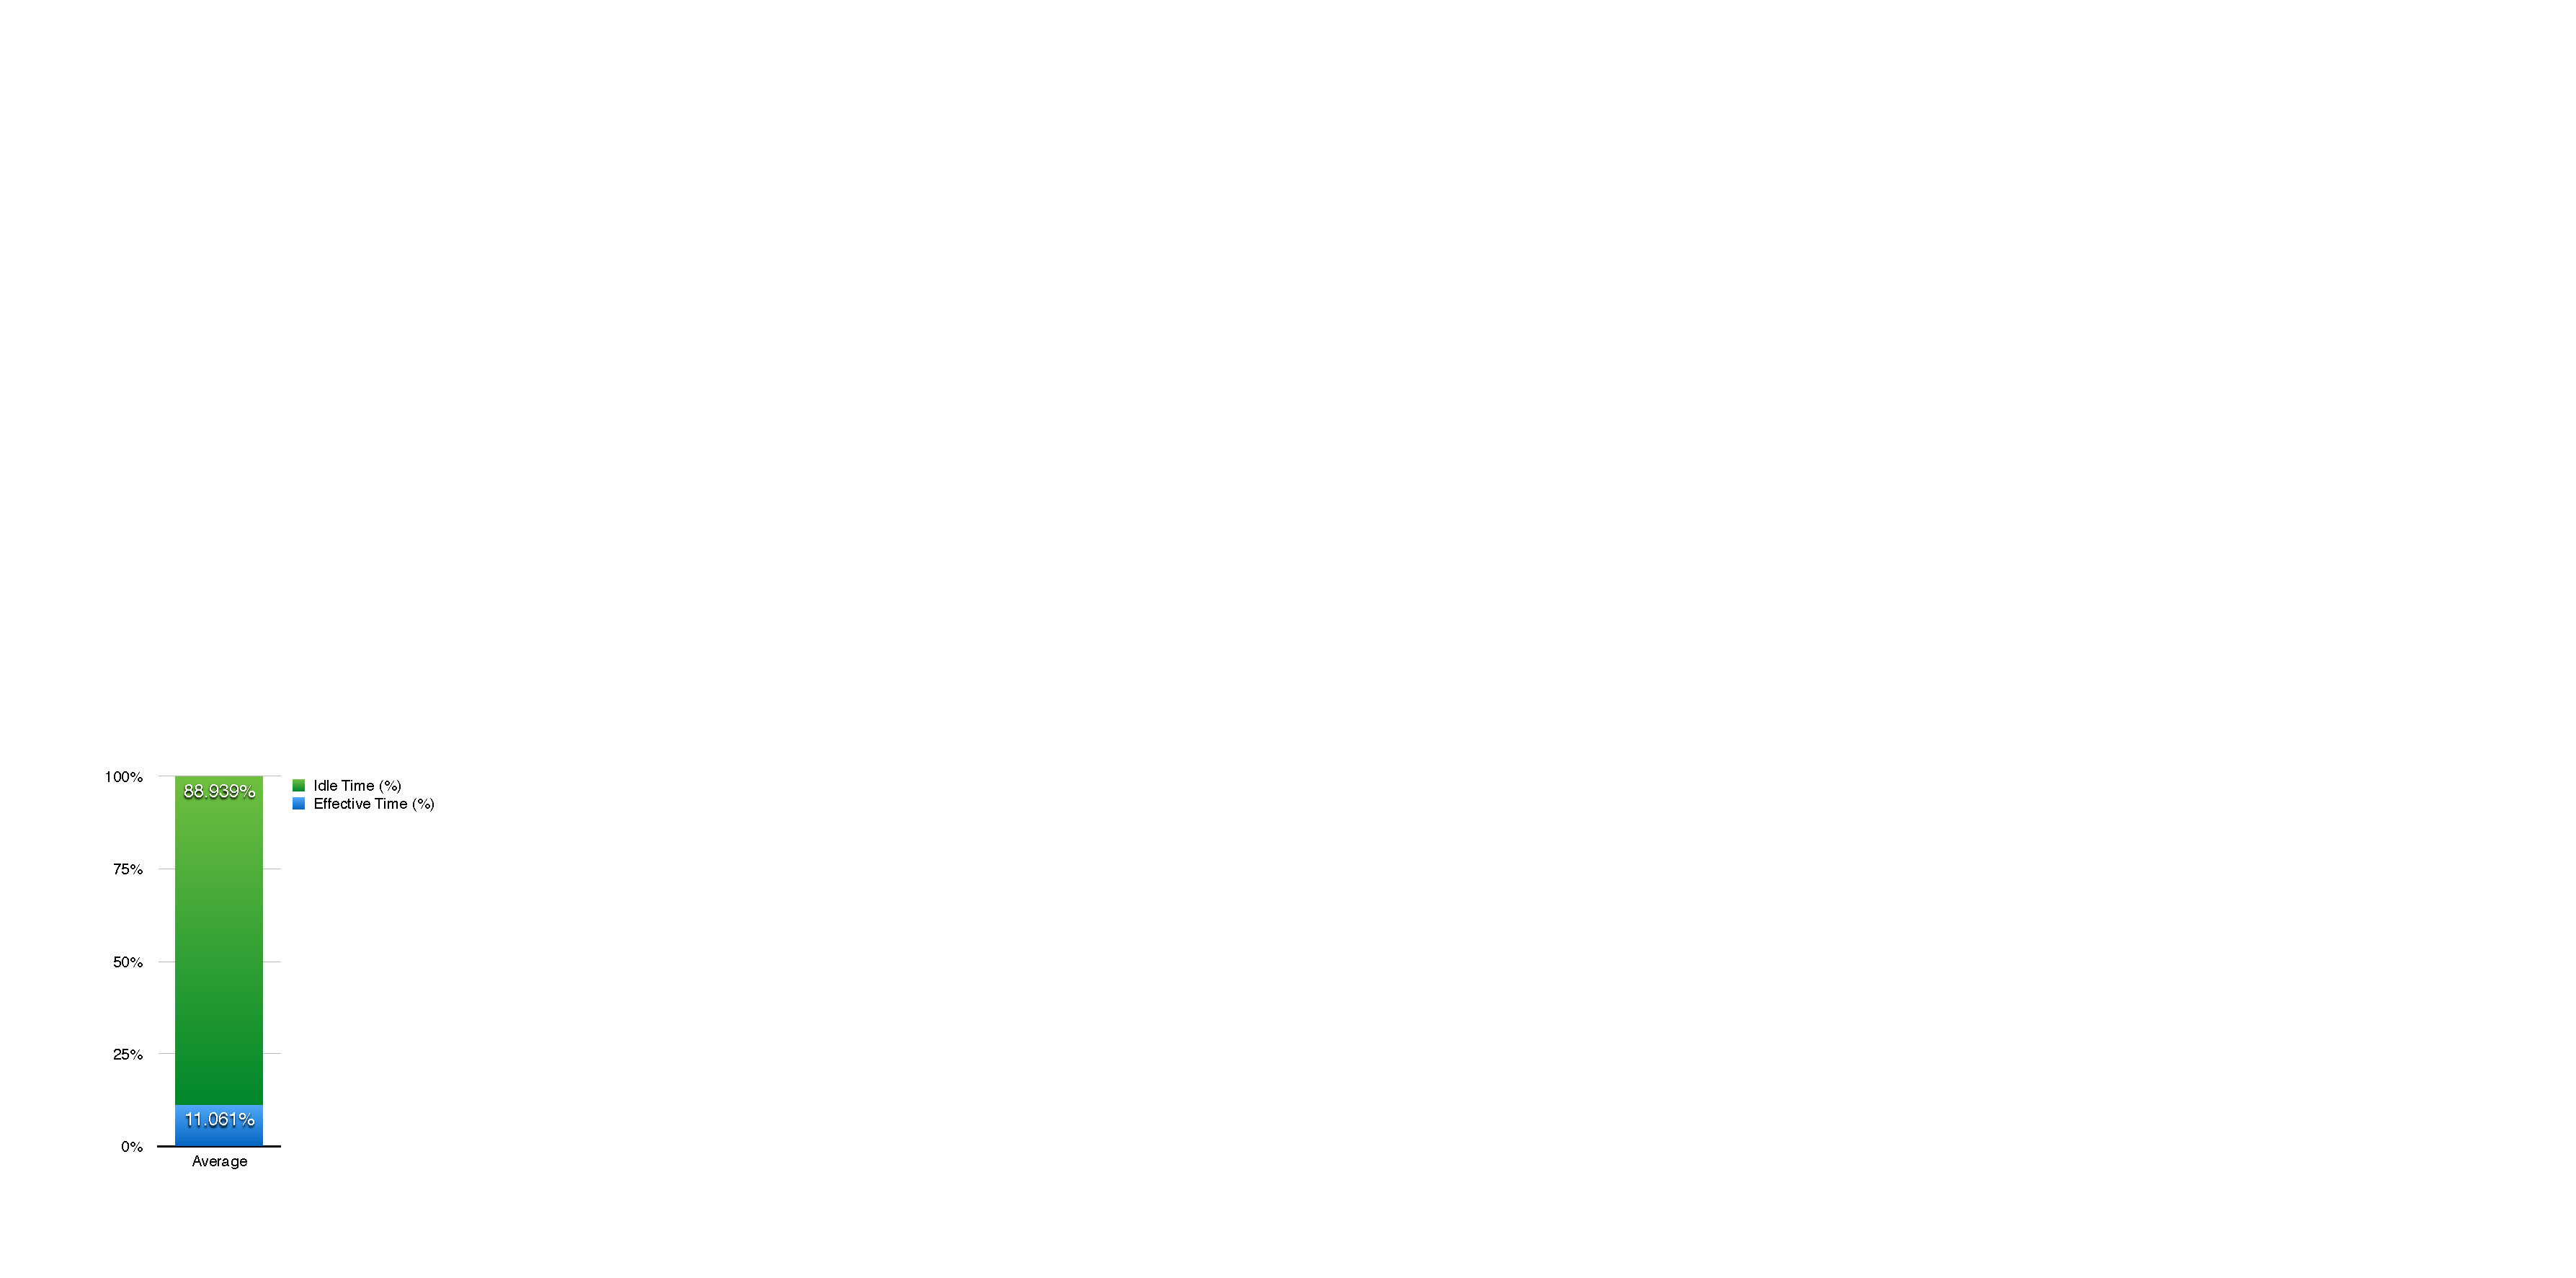
\includegraphics[height=\linewidth]{./images/cloud_ecspec_breakdown}
    \caption{Baseline Event Cycle: latency breakdown.}
    \label{fig:ecspecf_base}
  \end{subfigure}%
  % ECSpec fast cloud breakdown figure
  \begin{subfigure}{.5\textwidth}
    \centering
    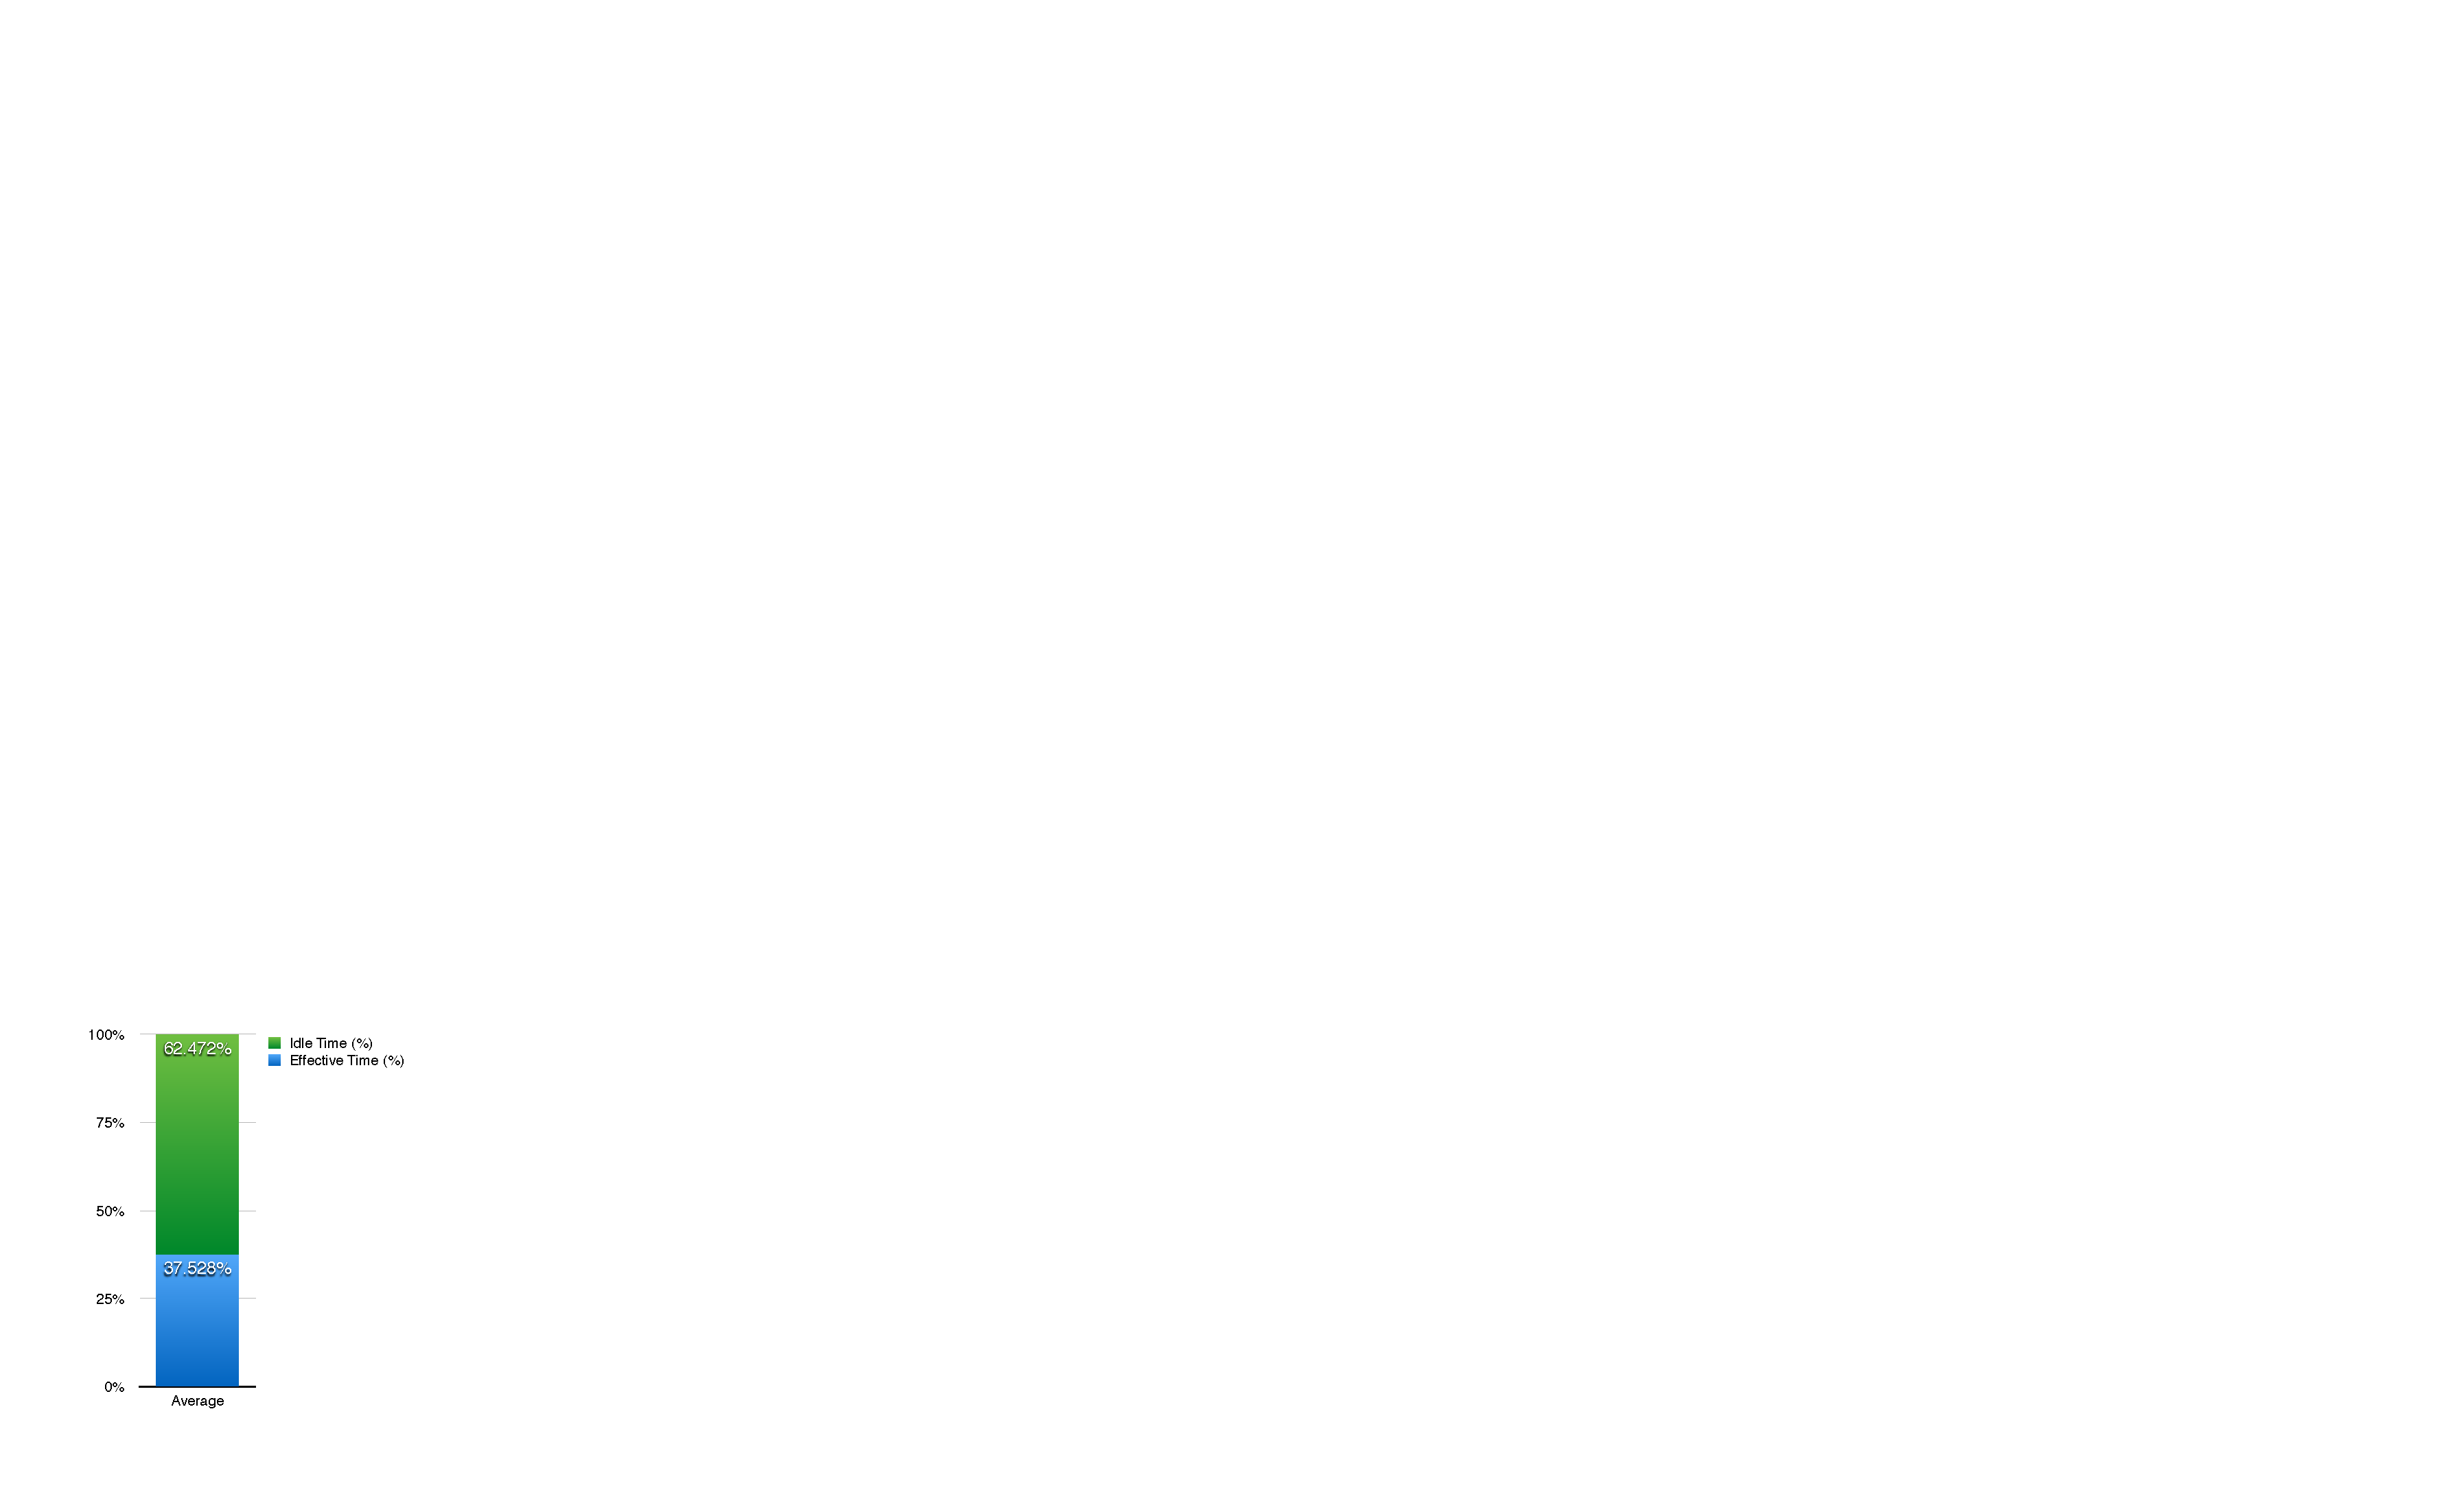
\includegraphics[height=\linewidth]{./images/cloud_ecspecf_breakdown}
    \caption{Half-period Event Cycle: latency breakdown.}
    \label{fig:ecspecf_half}
  \end{subfigure}
  \caption[Cloud-based approach: event latency breakdown.]{Cloud-based approach: Event Cycle latency breakdown.}
  \label{fig:ecspecf_breakdown}
\end{figure}

The graphs presented in Figure~\ref{fig:ecspecf_base} and Figure~\ref{fig:ecspecf_half} shows that
as in the previous experiment, during most of time of an \textit{Event Cycle} the \gls{ALE} module is
in an idle state. However, unlike in the previous experiment the \textit{ECspecs} affected the percentage of time
where \gls{ALE} is processing the events (\textit{Effective Time}) and where is in an idle state (\textit{Idle Time}).
With the \textit{Baseline ECspec} the \gls{ALE} remains $\approx89\%$ of the \textit{Event Cycle} period
in an idle state while when configured with the \textit{Half-period ECspec} this value decreases to
$\approx62\%$. This means that during the \textit{Event Cycle} period the \gls{ALE} module can be in
an idle state during 9 seconds when configured with the \textit{Baseline ECspec} while with the
\textit{Half-period ECspec} this value can last for 3 seconds.\\

% TODO: Maybe this can be removed???
\pagebreak

Figure~\ref{fig:ecspecf_effective_breakdown} presents the time breakdown for the stages of the
event processing pipeline. Figure~\ref{fig:ecspecf_effective_base} presents the how much time is spent
in each phase of the pipeline when the \gls{ALE} is configured with \textit{Baseline ECspec} and in
Figure~\ref{fig:ecspecf_effective_half} when it is configured with the \textit{Half-period ECspec}.\\

% Baseline ECspec effective time breakdown
\begin{figure}[ht!]
  \centering
  % ECSpec Fast local breakdown figure
  \begin{subfigure}{.5\textwidth}
    \centering
    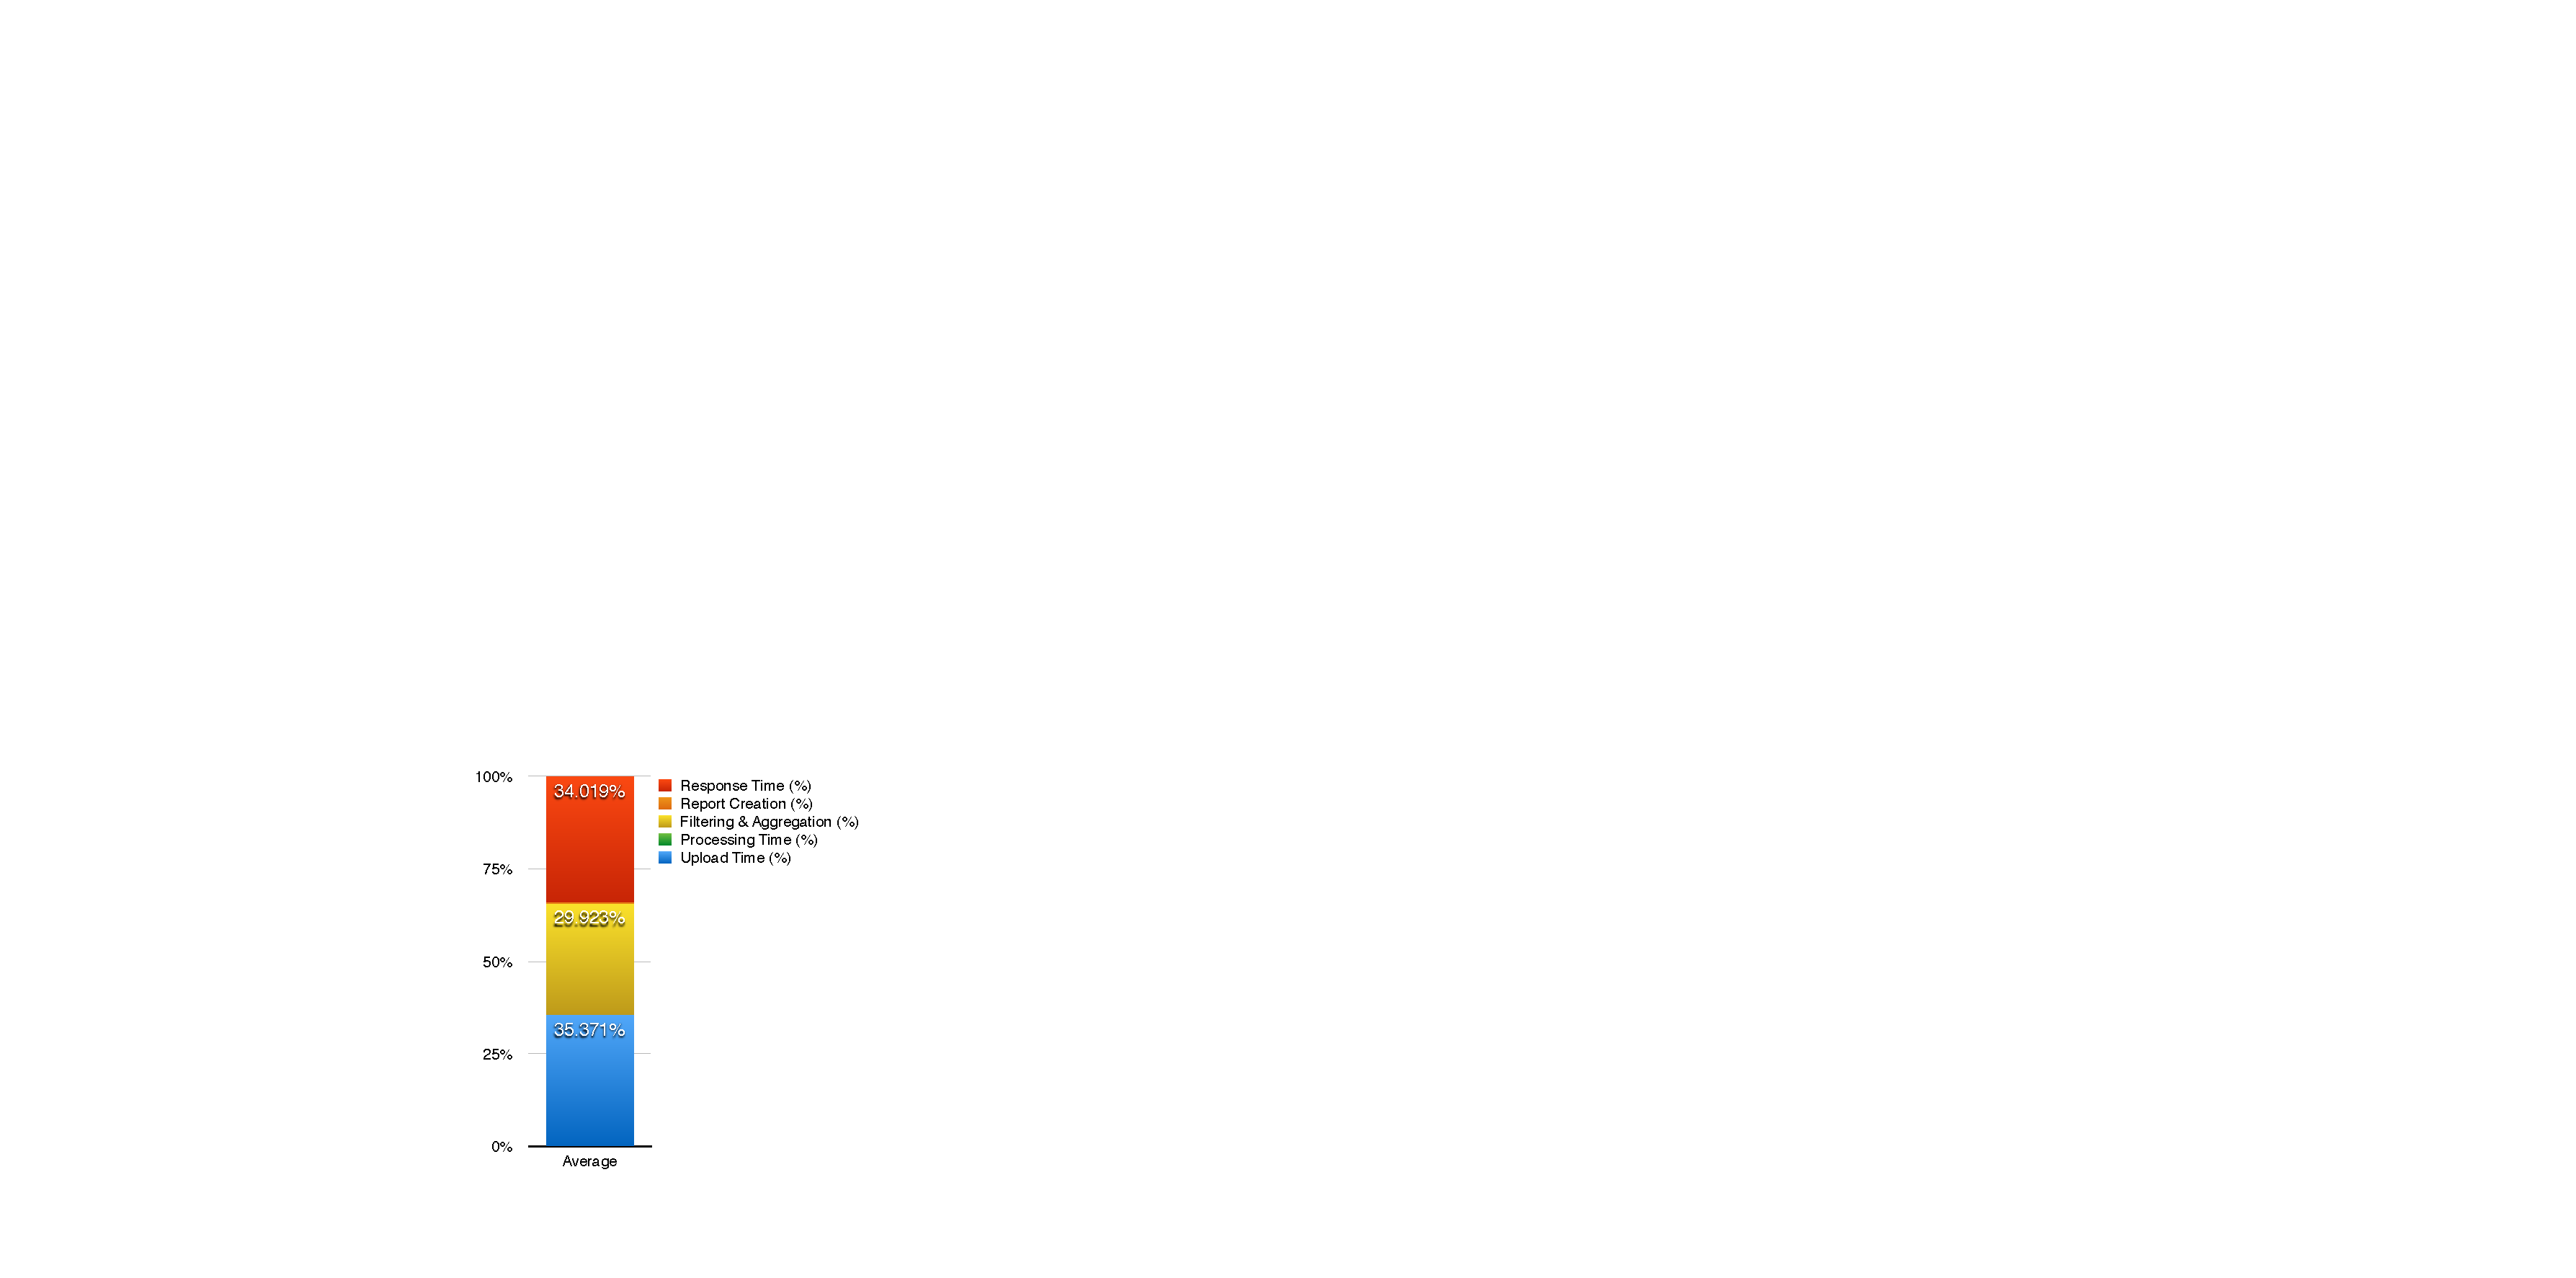
\includegraphics[height=\linewidth]{./images/cloud_ecspec_effective_breakdown}
    \caption{Baseline Event Cycle: event pipeline breakdown.}
    \label{fig:ecspecf_effective_base}
  \end{subfigure}%
  % ECSpec fast cloud breakdown figure
  \begin{subfigure}{.5\textwidth}
    \centering
    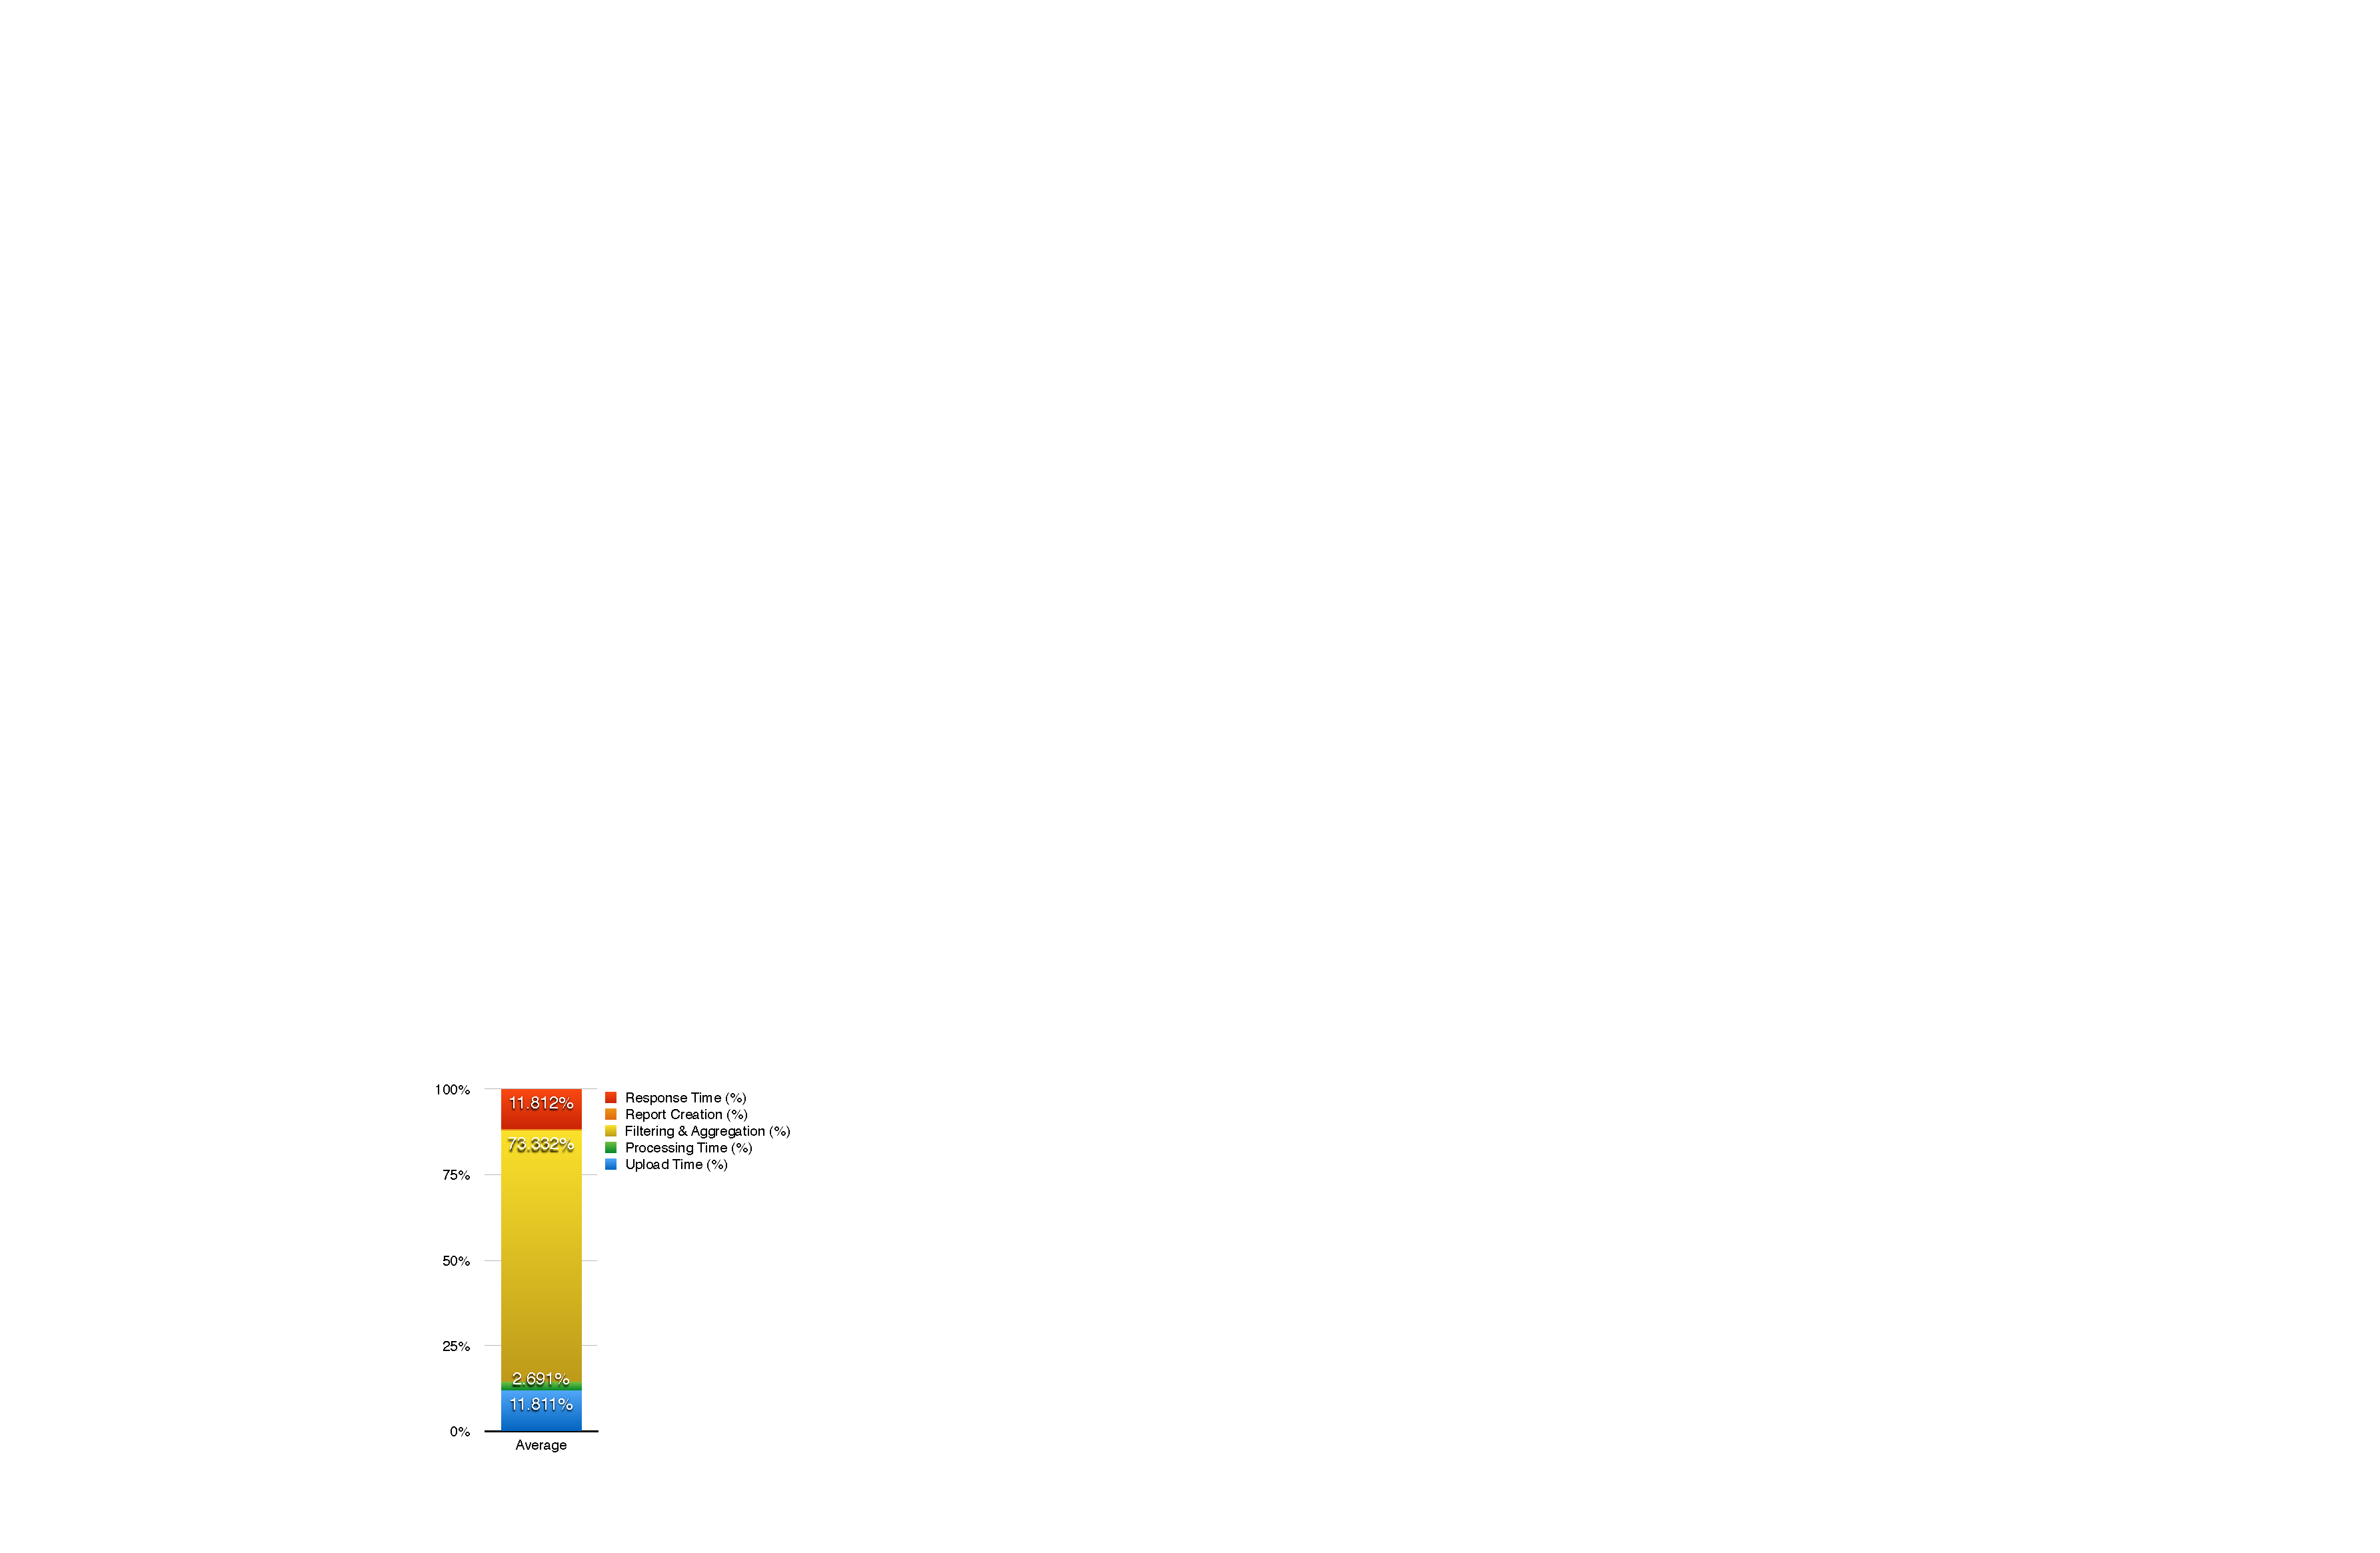
\includegraphics[height=\linewidth]{./images/cloud_ecspecf_effective_breakdown}
    \caption{Half-period Event Cycle: event pipeline breakdown.}
    \label{fig:ecspecf_effective_half}
  \end{subfigure}
  \caption[Cloud-based approach: event processing breakdown.]{Cloud-based approach: event processing pipeline breakdown.}
  \label{fig:ecspecf_effective_breakdown}
\end{figure}

Comparing the obtained results, it is possible to observe that time breakdown is evenly distributed
between the \textit{Upload} ($\approx35\%$), \textit{Filtering \& Aggregation} ($\approx30\%$) and
\textit{Response} ($\approx34\%$) stages when the \gls{ALE} module is configured with the \textit{Baseline ECspec},
while the \textit{Tag Porcessing} and \textit{Report Creation} stages represents a small percentage of the
total time, less than $\approx1\%$. When the \gls{ALE} is configured with the \textit{Half-period ECspec},
the \textit{Filtering \& Aggregation} stage is the most time consuming, representing close to $\approx 75\%$
of the total time. As when configured with the \textit{Baseline ECspec}, the \textit{Upload} and
\textit{Reponse} stages presents similar results, respectively close to $\approx10\%$ and $\approx11\%$.
Regarding the \textit{Processing} stage, as in the fog-based approach the time required to process the
event data increased in a significant way, from less than $\approx0.3\%$ to $\approx3\%$. The
\textit{Report Creation} stage presented the same values from the previous configuration ($\approx0.3\%$).\\

As in the previous experiment the event latency presented a better overall performance for the faster \textit{ECspec}.
According the metric values presented in Table~\ref{table:cloud_metrics} it is possible to observe that the event
latency decrease from 8.244s to 4.266s. The values for the network latency improved when the \gls{ALE} is
configured with the faster \textit{ECspec}, close to $\approx65\%$ of improvement for the \textit{Upload Latency}
metric - from 0.294s to 0.101s - and $\approx40\%$ for the \textit{Response Latency} metric -
from 0.228s to 0.138s. The values for the time where the \gls{ALE} remains in an idle state also presented
a significant improvement, from 7.346s to 2.569s.\\

\begin{table}[ht!]
  \centering
    \begin{tabular}{|l|c|c|}
    \hline
    Metric                        & Base Event Cycle & Half-period Event Cycle \\ \hline
    Upload Latency                & 0.294s           & 0.103s                  \\ \hline
    Tag Processing Latency        & 0.002s           & 0.024s                  \\ \hline
    Idle Processing Latency       & 7.346s           & 2.569s                  \\ \hline
    Filter \& Aggregation Latency & 0.370s           & 1.490s                  \\ \hline
    Report Creation Latency       & 0.003s           & 0.003s                  \\ \hline
    Response Latncy               & 0.228s           & 0.149s                  \\ \hline
    Event Latency                 & 8.244s           & 4.266s                  \\ \hline
    \end{tabular}
  \caption[Cloud-based approach: performance results.]{Cloud-based approach: performance metrics results.}
  \label{table:cloud_metrics}
\end{table}

As in the fog-based approach the value for the \textit{Tag Processing Latency} increased $\approx1000\%$ when
the \gls{ALE} is configured with \textit{Half-period ECspec} - from 0.002s to 0.024s. Unlike in the
previous experiment, the value for the \textit{Filtering \& Aggregation Latency} metric increased $\approx300\%$
- from 0.370s to 1.490s.

% Fog-based warehouse latency
\subsubsection{Fog-based warehouse latency}
\label{subs:eval_exp_latency_ecspec}
Figure~\ref{fig:ecspec_breakdown} summarizes the latency breakdown for an event that occurs in a fog-based
smart warehouse. Figure~\ref{fig:ecspec_base} shows the latency breakdown for an event when the
\gls{ALE} module is configured with the \textit{Baseline ECspec} and in Figure~\ref{fig:ecspec_half}
when it is configured with the \textit{Half-period ECspec}.\\

% Baseline ECspec event time breakdown
\begin{figure}[ht!]
 % ECSpec local breakdown figure
 \centering
 \begin{subfigure}{.5\textwidth}
   \centering
   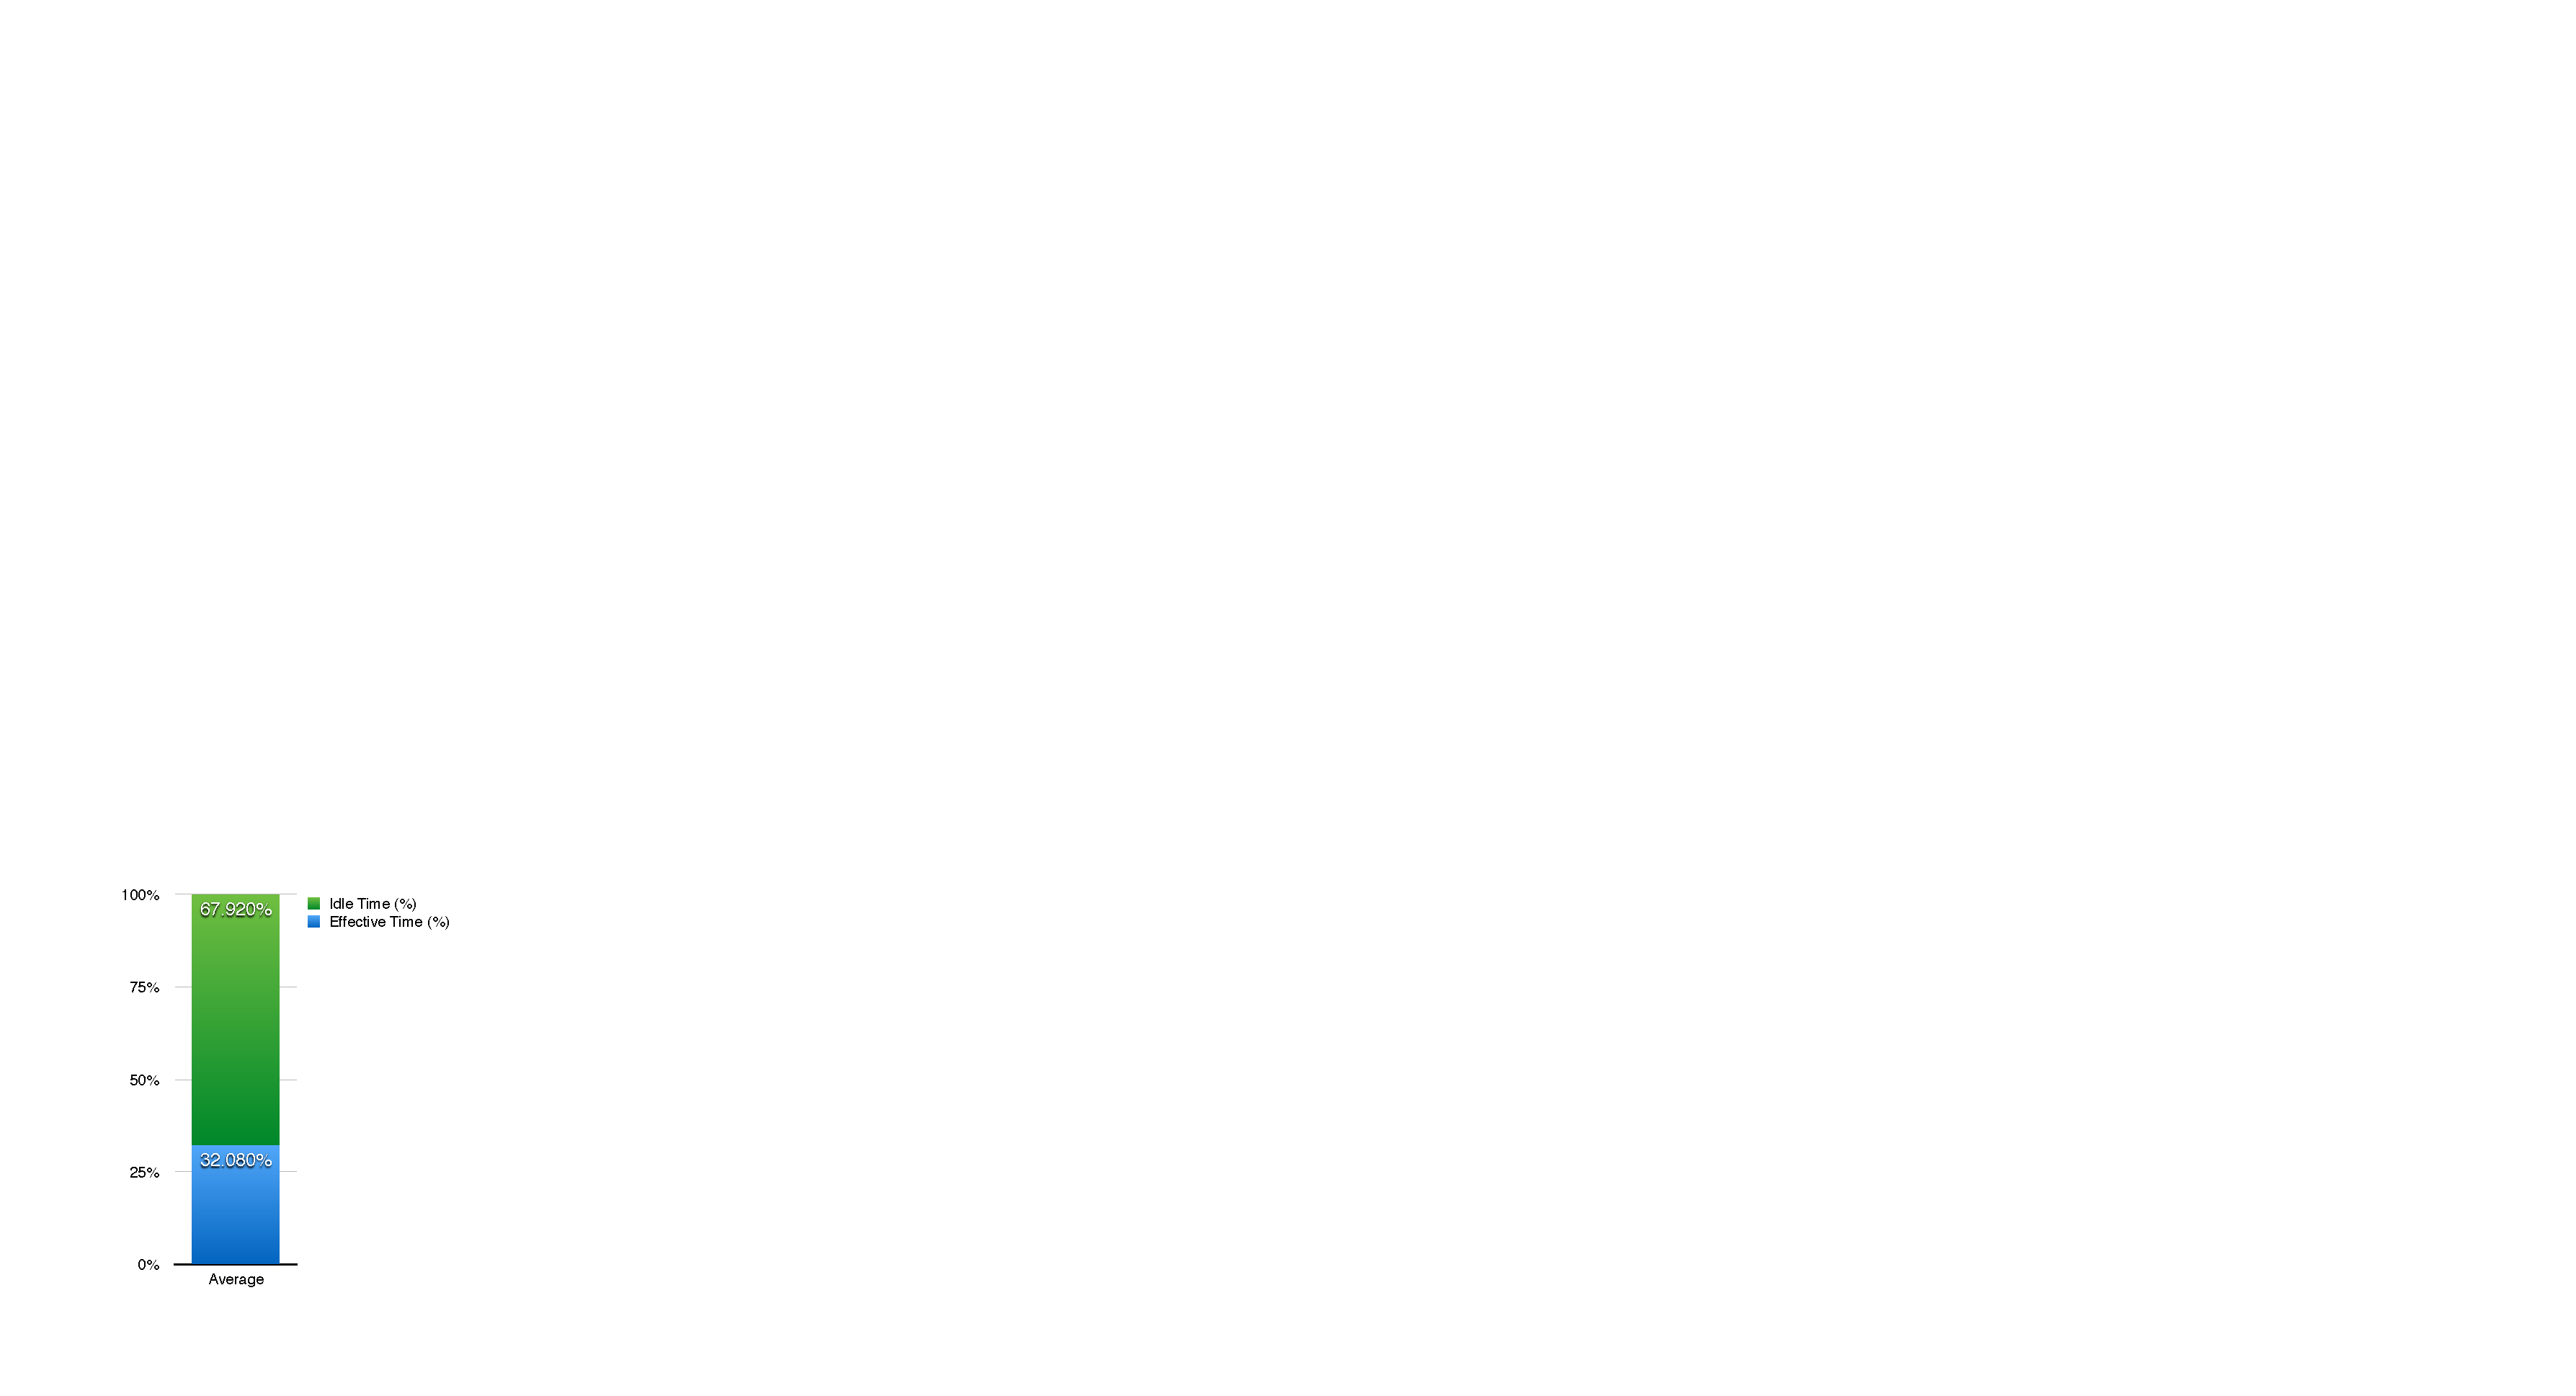
\includegraphics[height=\linewidth]{./images/edge_ecspec_breakdown}
   \caption{Baseline Event Cycle: latency breakdown.}
   \label{fig:ecspec_base}
 \end{subfigure}%
 % ECSpec cloud breakdown figure
 \begin{subfigure}{.5\textwidth}
   \centering
   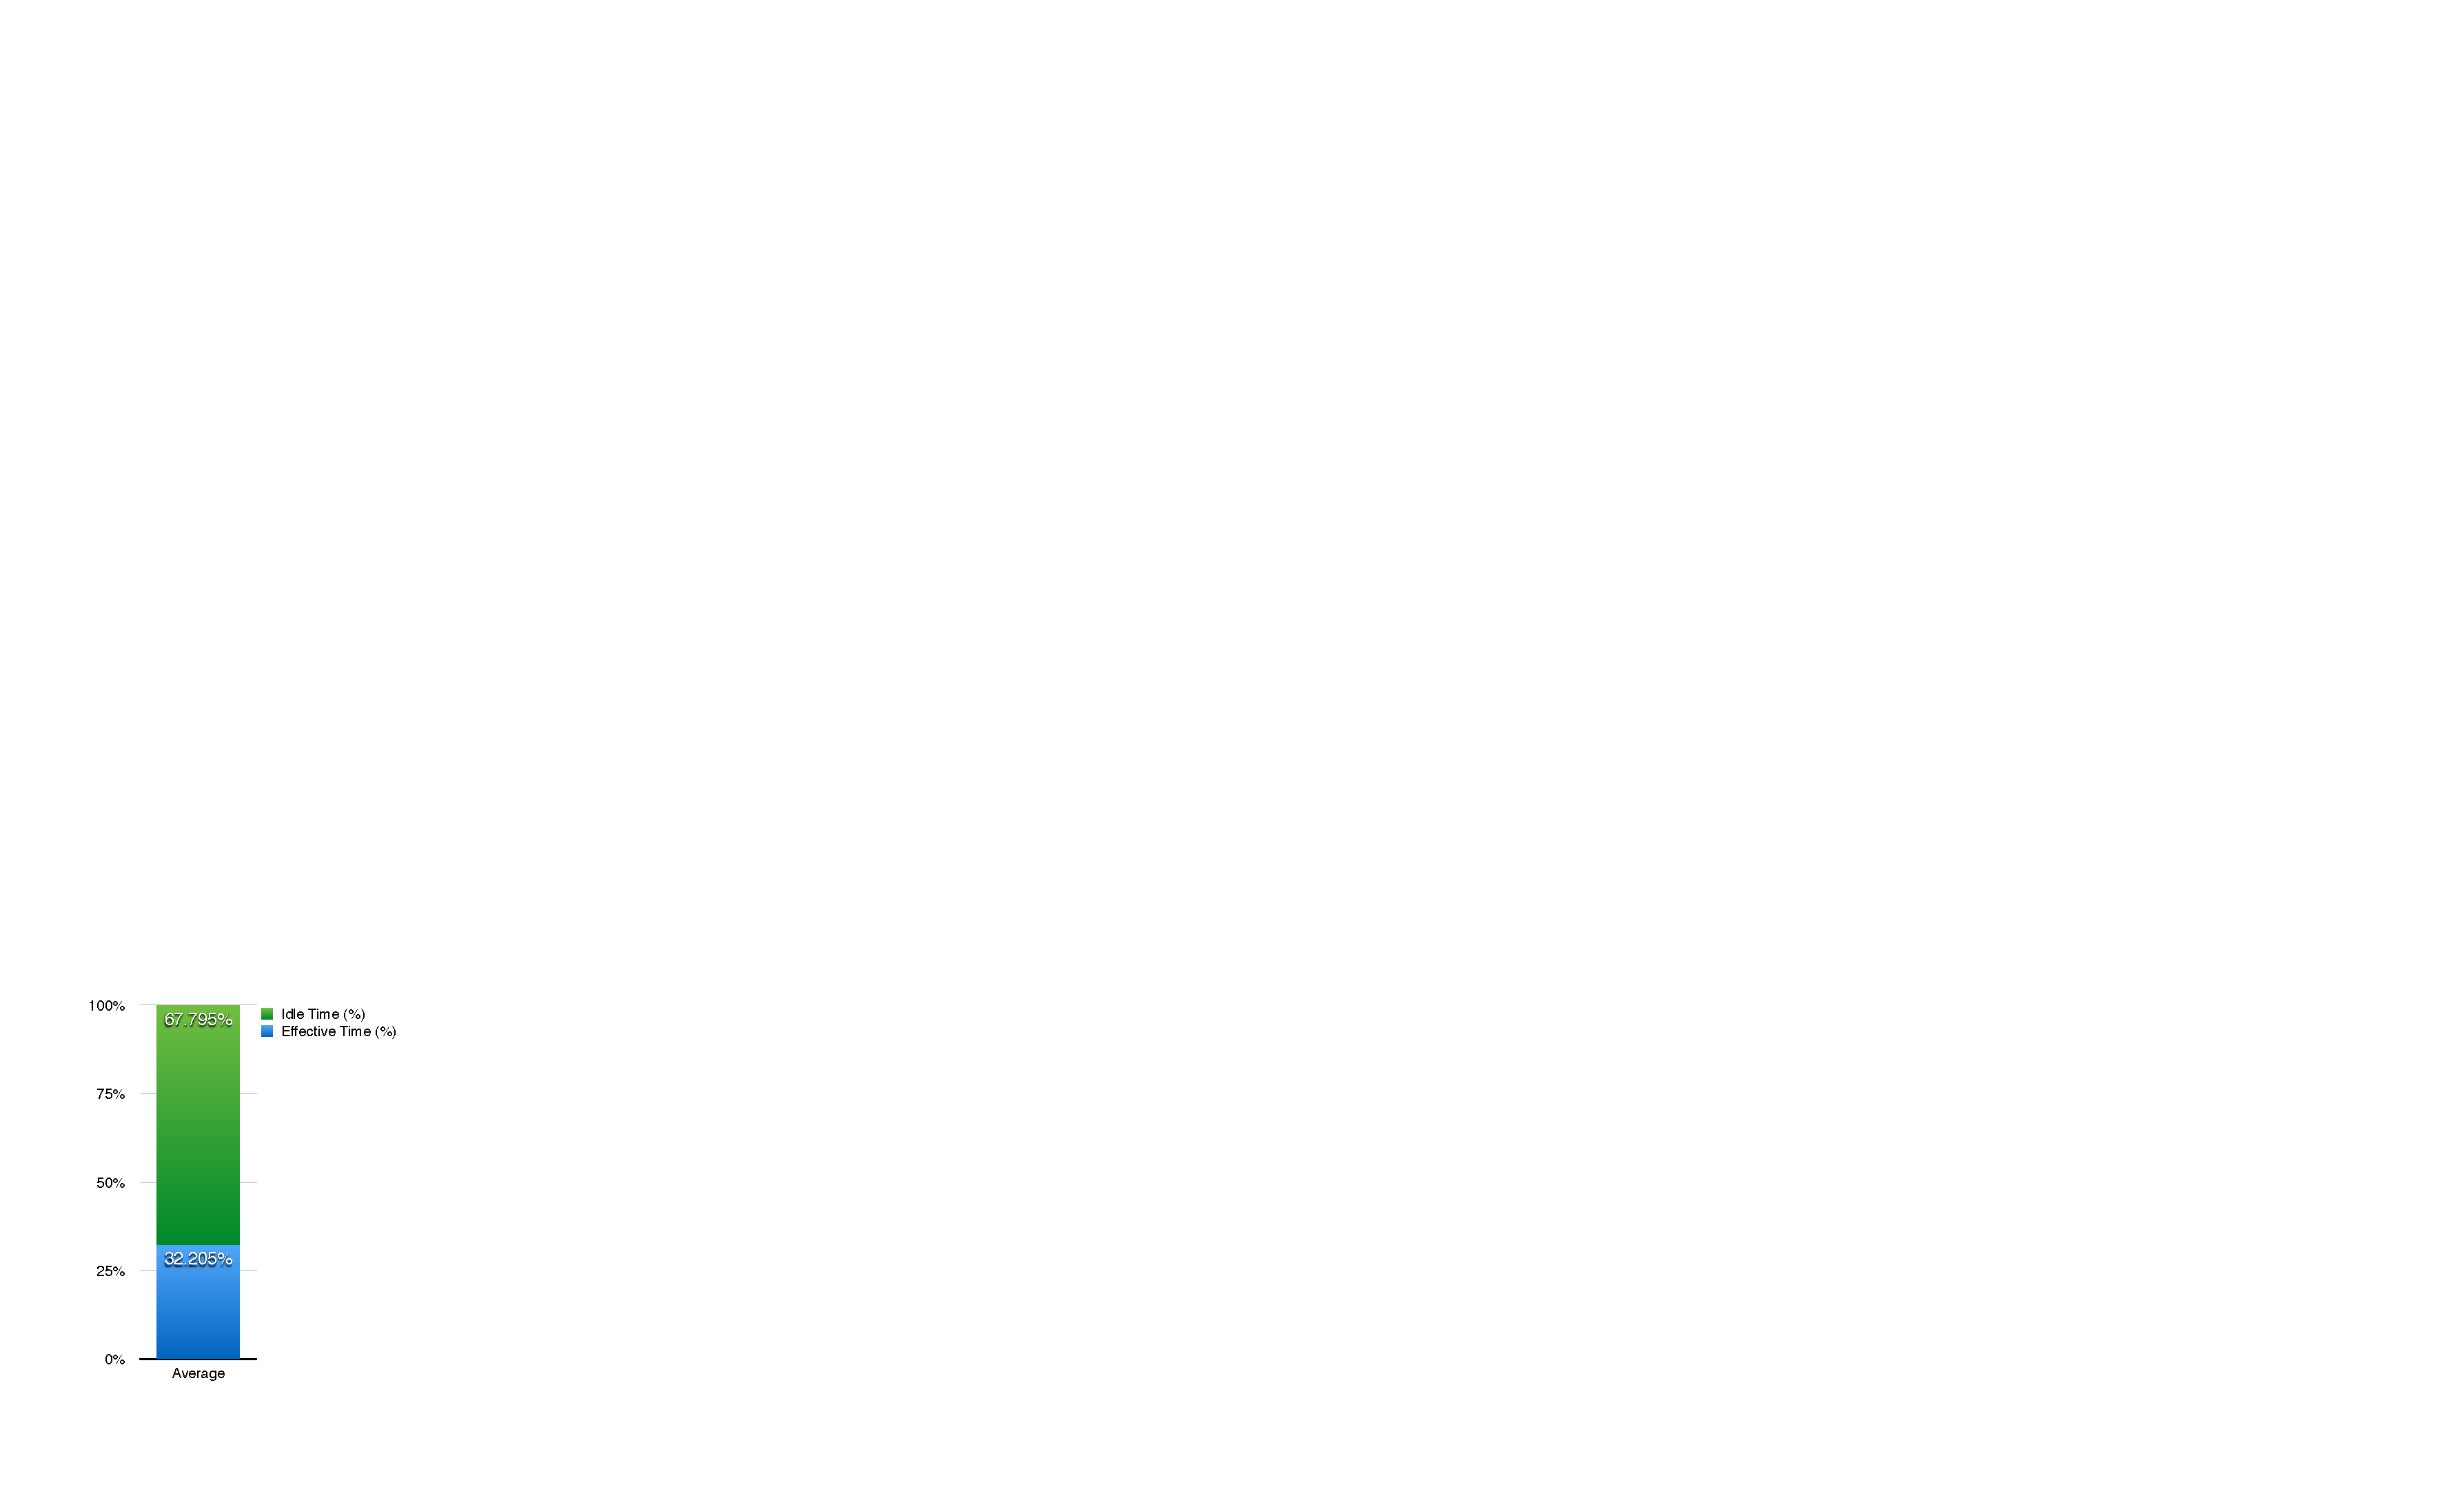
\includegraphics[height=\linewidth]{./images/edge_ecspecf_breakdown}
   \caption{Half-period Event Cycle: latency breakdown.}
   \label{fig:ecspec_half}
 \end{subfigure}
 \caption[Fog-based approach: event latency breakdown.]{Fog-based approach: Event Cycle latency breakdown.}
 \label{fig:ecspec_breakdown}
\end{figure}

Comparing the graphs for both \textit{ECspecs} is possible to conclude that during most of the time of
an \textit{Event Cycle} the \gls{ALE} module is in an idle state (\textit{Idle Time}) - close to $\approx68\%$
in both configurations - while in the remaining time the \gls{ALE} is processing the event that was
collected (\textit{Effective Time}). Considering the duration of the \textit{ECspecs} it means that in
average when the \gls{ALE} is configured with the \textit{Baseline ECspec} the module can be in an idle
state during 7s while with the \textit{Half-period ECspec} this idle state can last for 3 seconds.\\

Figure~\ref{fig:ecspec_effective_breakdown} summarizes how the time is spent during the stages of the
event processing pipeline. Figure~\ref{fig:ecspec_effective_base} presents the time breakdown for
each stage of the pipeline when the \gls{ALE} is configured with \textit{Baseline ECspec} and in
Figure~\ref{fig:ecspec_effective_half} when it is configured with the \textit{Half-period ECspec}.\\

% Baseline ECspec effective time breakdown
\begin{figure}[ht!]
  % ECSpec local breakdown figure
  \centering
  \begin{subfigure}{.5\textwidth}
    \centering
    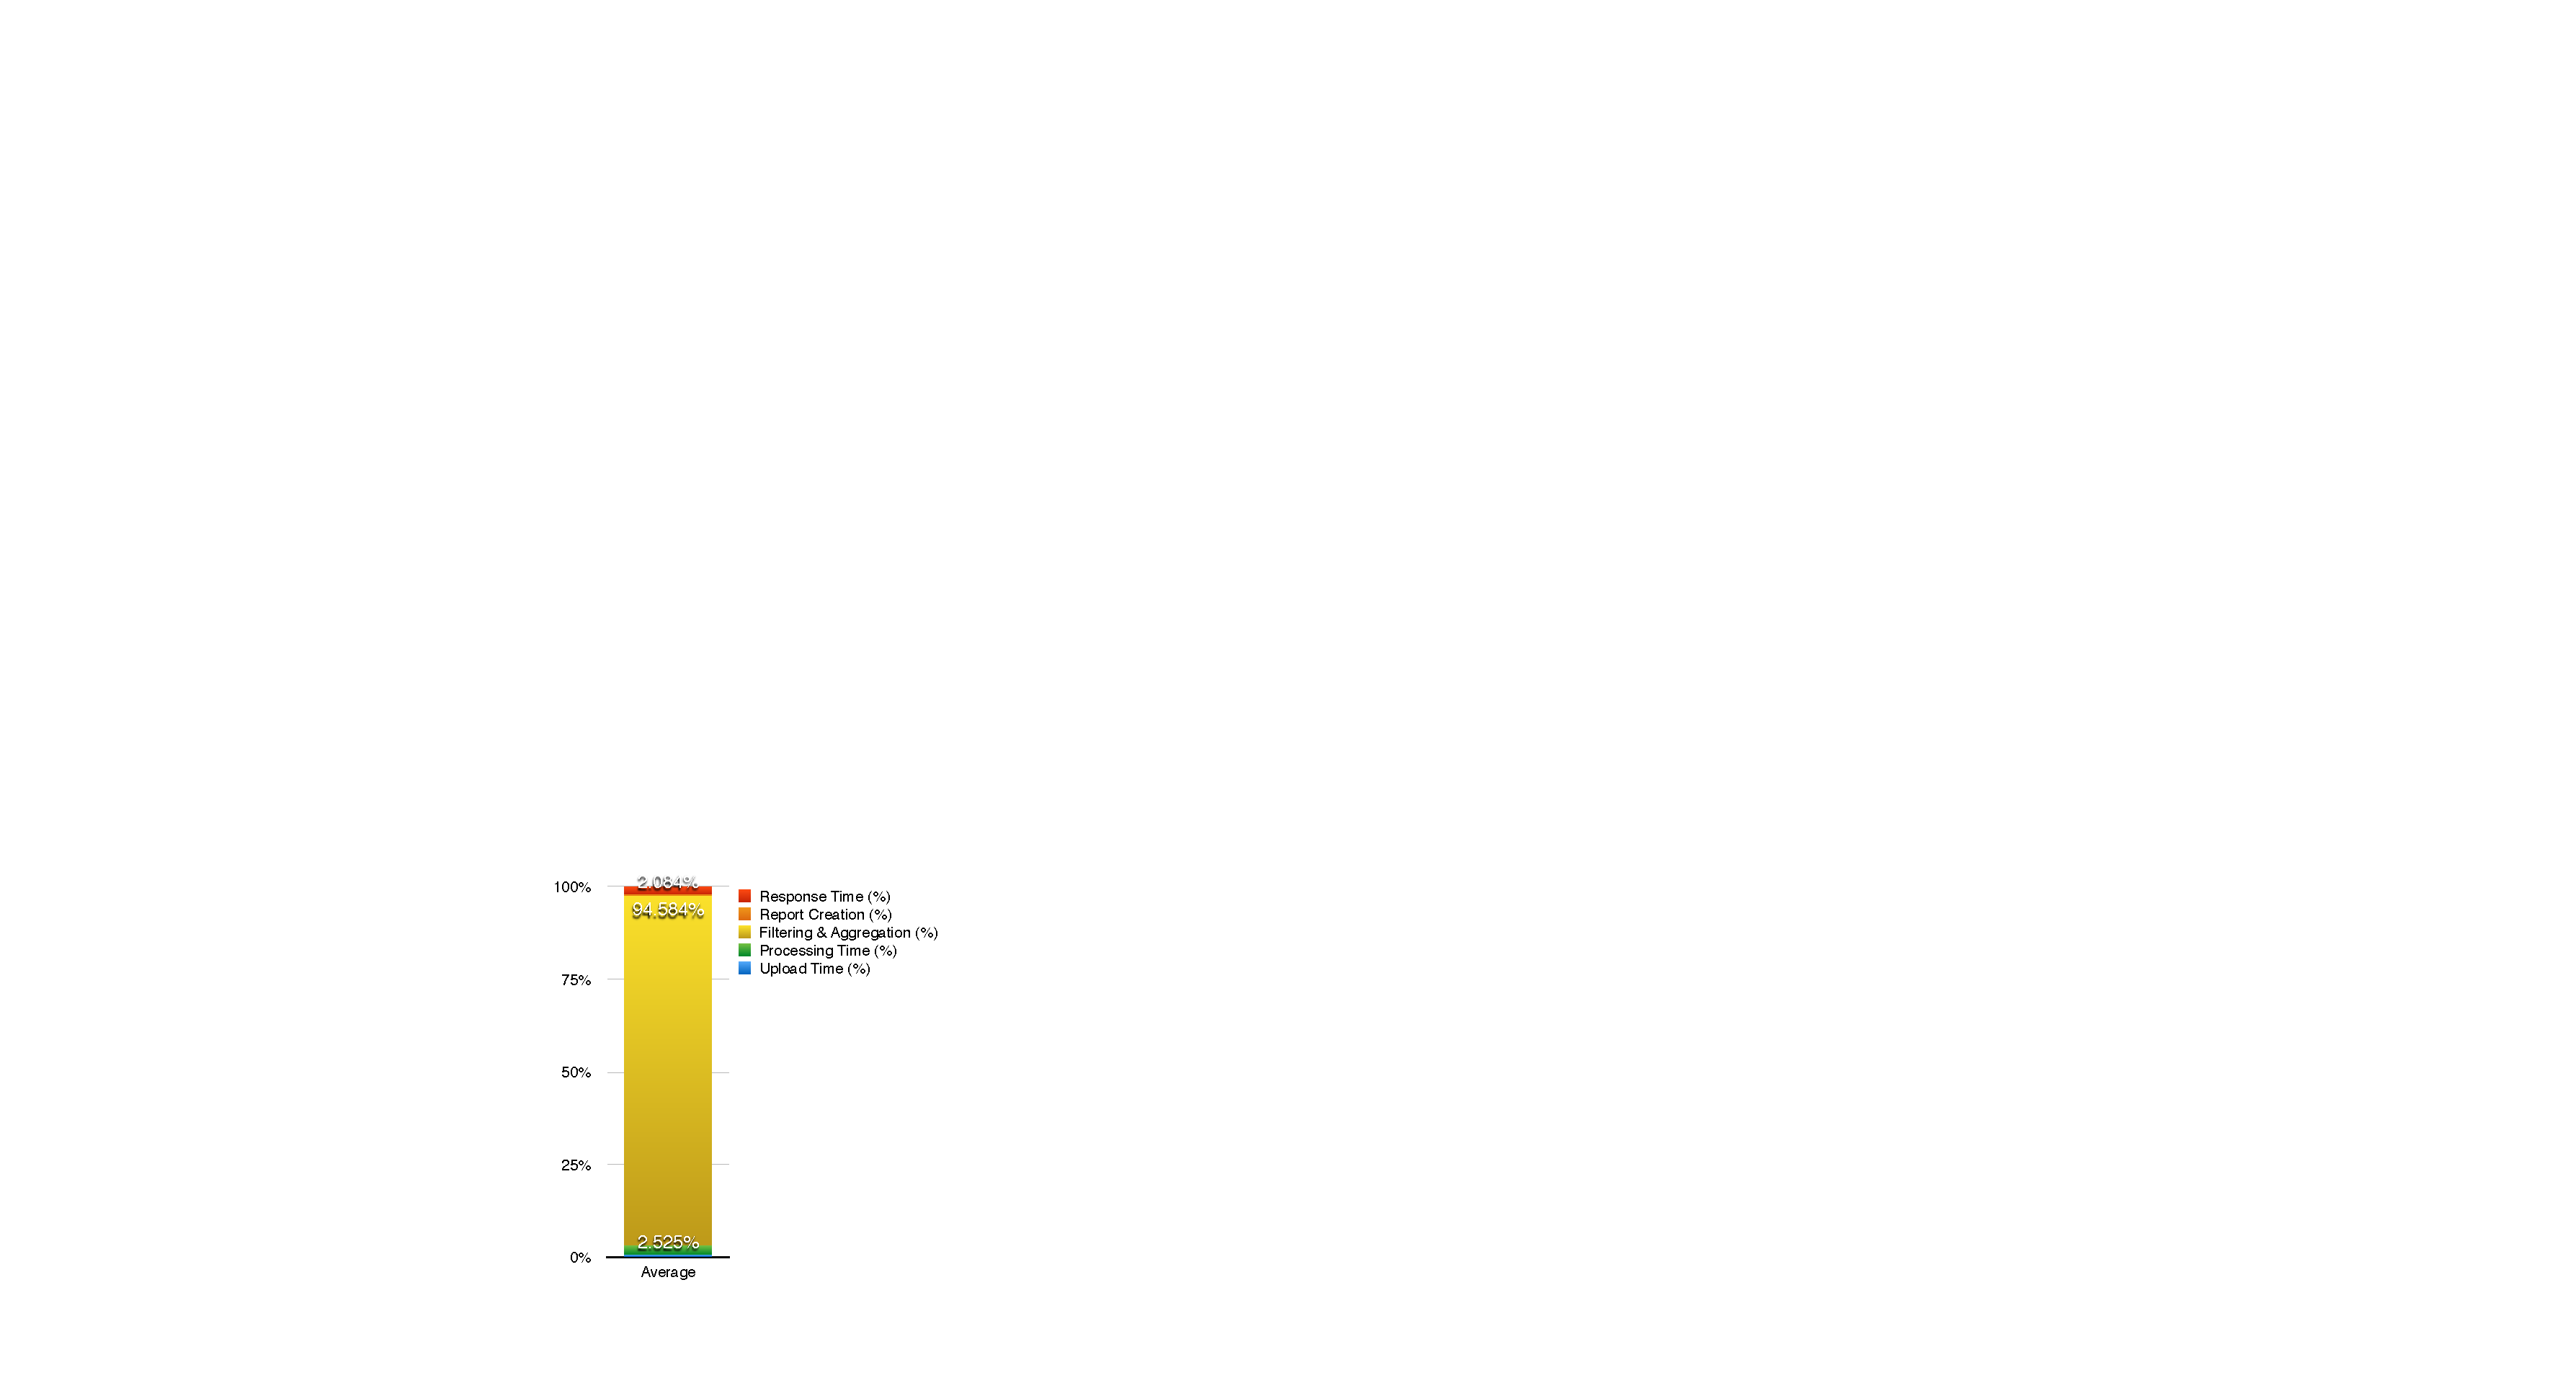
\includegraphics[height=\linewidth]{./images/edge_ecspec_effective_breakdown}
    \caption{Baseline Event Cycle: event pipeline breakdown.}
    \label{fig:ecspec_effective_base}
  \end{subfigure}%
  % ECSpec cloud breakdown figure
  \begin{subfigure}{.5\textwidth}
    \centering
    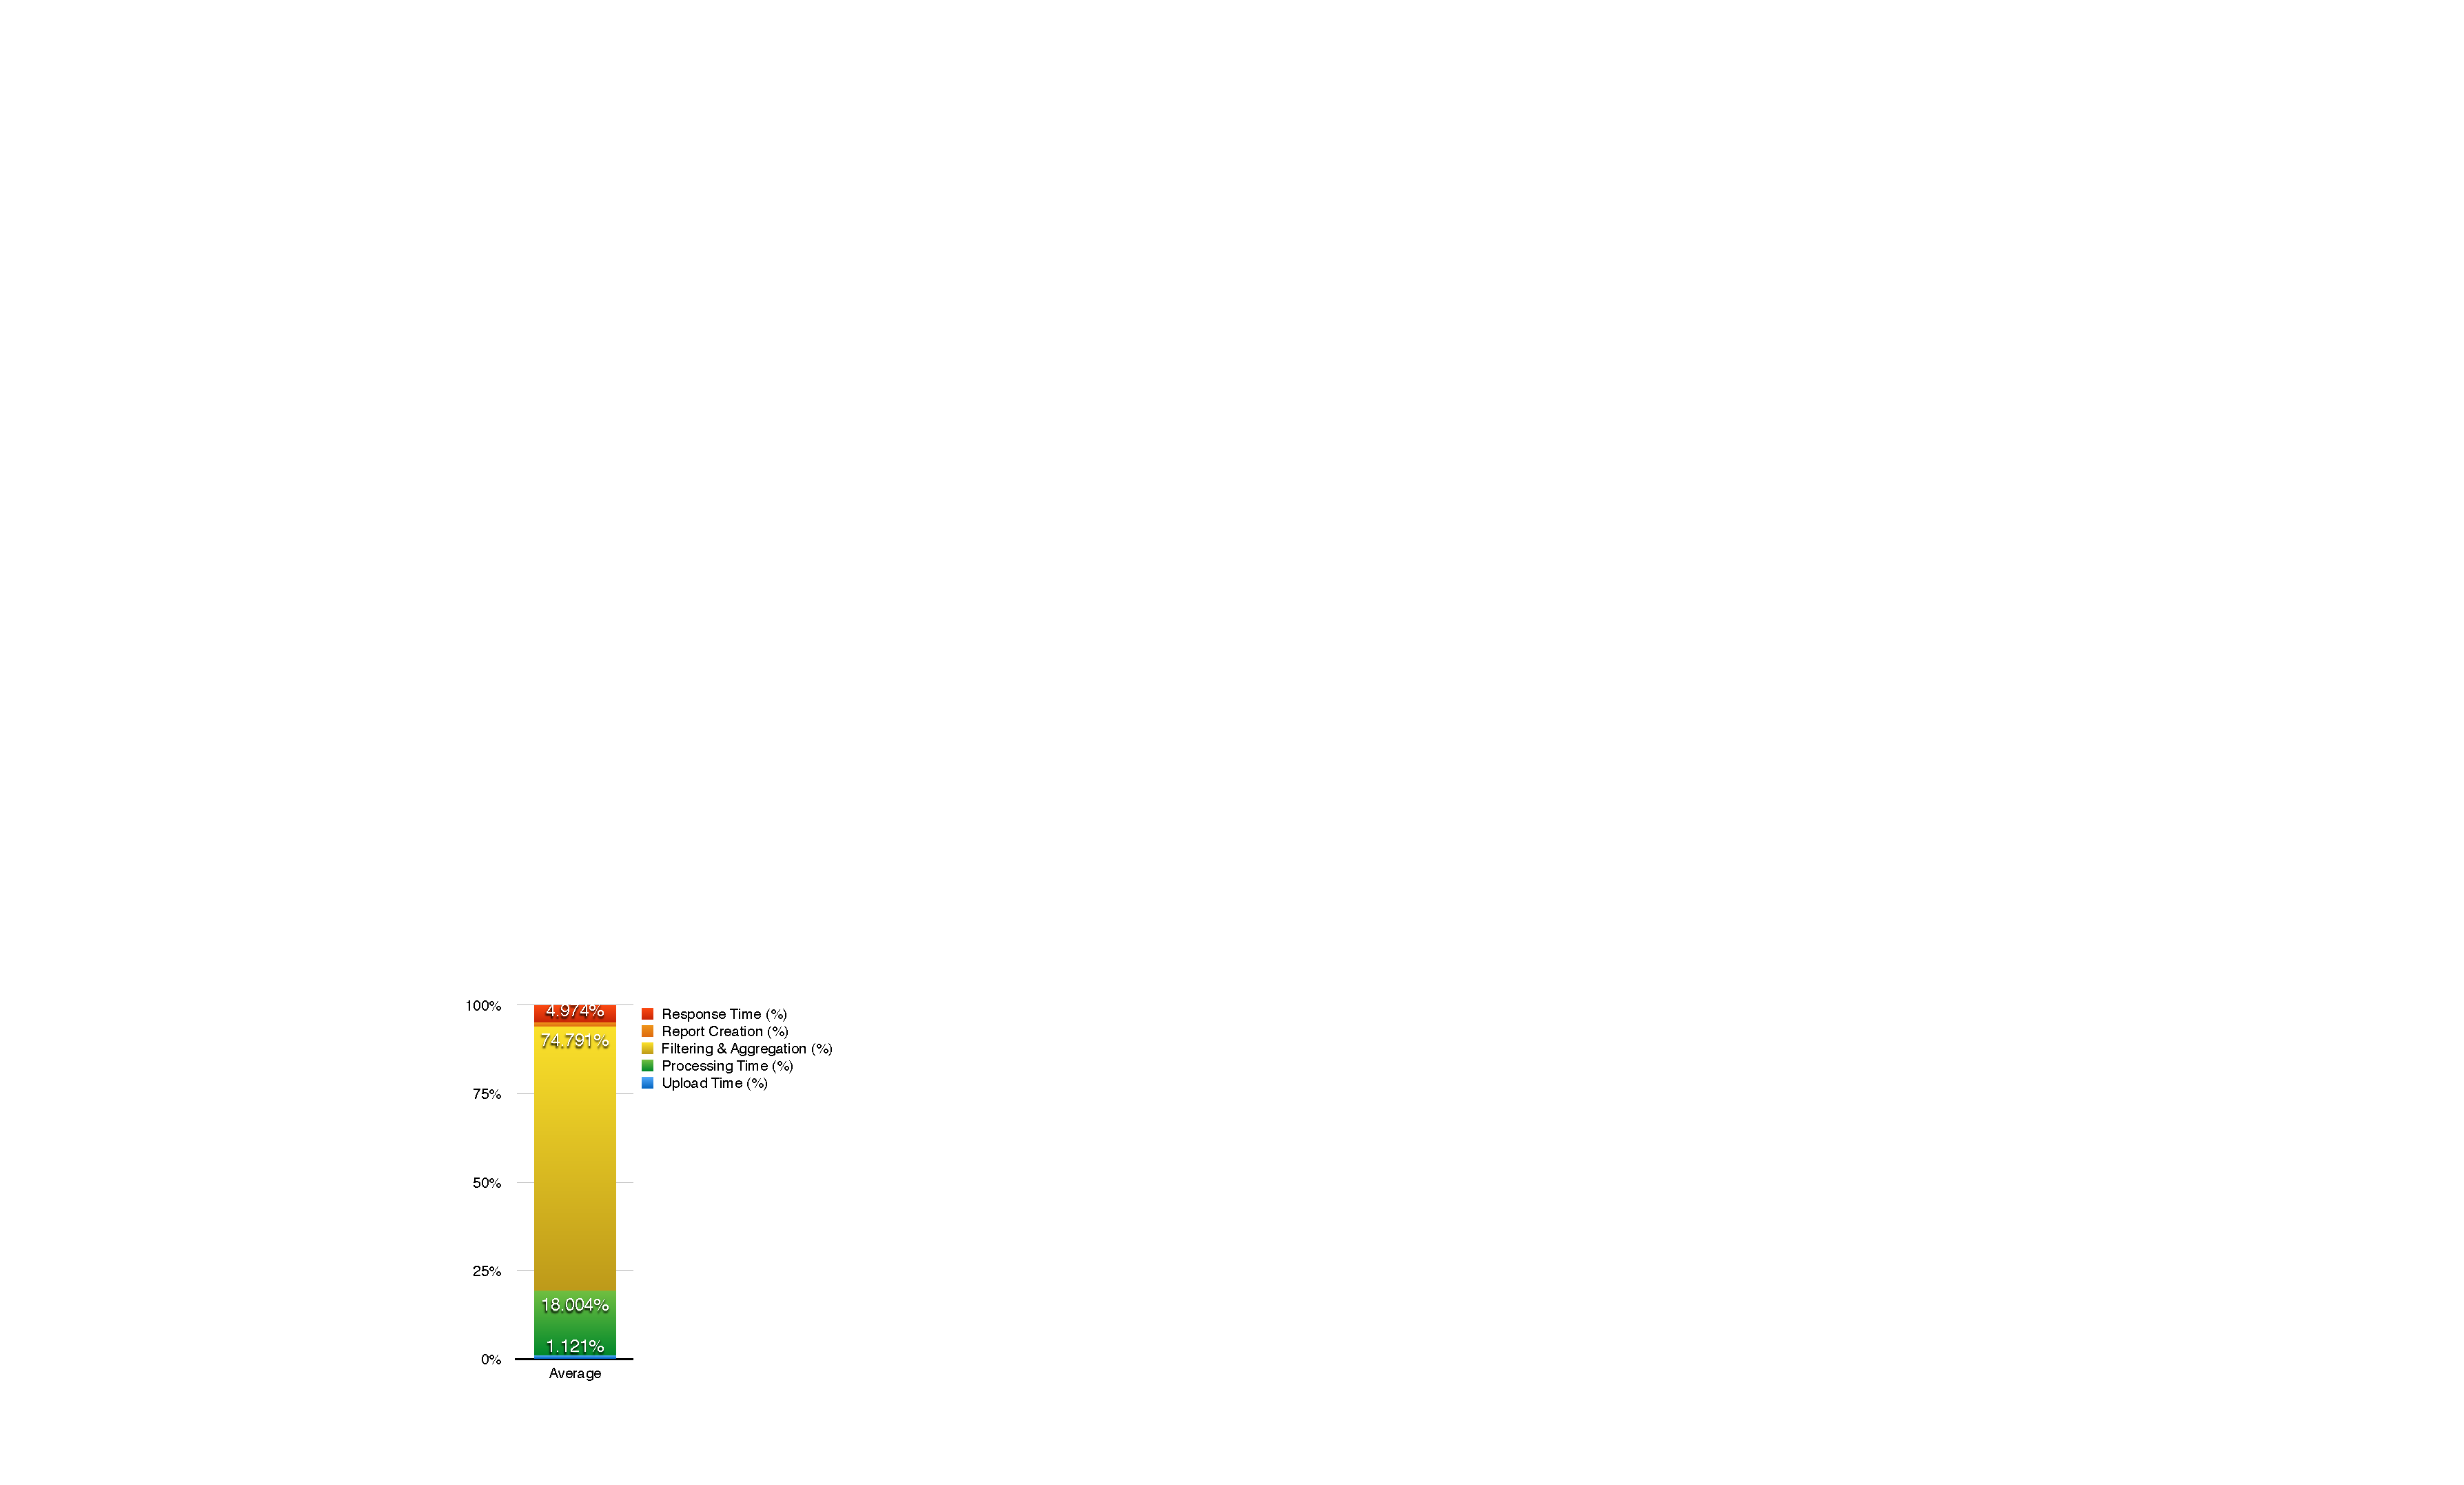
\includegraphics[height=\linewidth]{./images/edge_ecspecf_effective_breakdown}
    \caption{Half-period Event Cycle: event pipeline breakdown.}
    \label{fig:ecspec_effective_half}
  \end{subfigure}
  \caption[Fog-based approach: event processing breakdown.]{Fog-based approach: event processing pipeline breakdown.}
  \label{fig:ecspec_effective_breakdown}
\end{figure}

It is possible to observe that the \textit{Fltering \& Aggregation} stage is the most time consuming
for both \textit{Event Cycle} specifications. With the \textit{Baseline ECspec} this stage occupies
close to $\approx95\%$ of the total time, while with the \textit{Half-period ECspec} this value is
close to $\approx75\%$. The reason for this difference is in the \textit{tag Processing Latency} stage.
With the \textit{Baseline ECspec} the time to processing the event data represents close to $\approx2.5\%$
of the total time while with the \textit{Half-period ECspec} this value is close to $\approx18\%$.
The \textit{Upload} and \textit{Response} latency together represents a small percentage of
the time spent to process the event - close to $\approx5\%$ for both specifications - while the percentage
of time to create the reports represents less than $\approx1\%$ of the total time.\\

The behavior expected when the \gls{ALE} is configured with a faster \textit{Event Cycle} specification
is that the event latency presents a better overall performance. According the metric values presented in
Table~\ref{table:fog_metrics} it is possible to observe that the event latency improves in a significant
way - from 7.450s to 4.250s. This result is achieved thanks to the improvement in the latency
of at the \textit{Filtering \& Aggregation Latency} by $\approx52\%$ - from 2.530s to 1.230s - and the
amount of time that \gls{ALE} is in an idle state - from 4.944s to 2.747s. Regarding the network
latency, the values for the \textit{Upload Latency} and \textit{Response Latency} improved 1ms for both
metrics.\\

% Metrics Result
\begin{table}[ht!]
  \centering
    \begin{tabular}{|l|c|c|}
    \hline
    Metric                            & Base Event Cycle & Half-period Event Cycle \\ \hline
    Upload Latency                    & 0.005s           & 0.004s                  \\ \hline
    Tag Processing Latency            & 0.049s           & 0.279s                  \\ \hline
    Idle Processing Latency           & 4.944s           & 2.747s                  \\ \hline
    Filter \& Aggregation Latency     & 2.530s           & 1.203s                  \\ \hline
    Report Creation Latency           & 0.001s           & 0.003s                  \\ \hline
    Response Latency                  & 0.010s           & 0.009s                  \\ \hline
    Event Latency                     & 7.540s           & 4.245s                  \\ \hline
    \end{tabular}
  \caption[Fog-based approach: performance results.]{Fog-based approach: performance metrics results.}
  \label{table:fog_metrics}
\end{table}

However, when configured with a faster \textit{Event Cycle} specification the tag processing time
presented an inferior performance, where time to process the event data increases $\approx470\%$
- from 0.049s to 0.279s. Also the report creation time increased $300\%$ - from 0.001s to 0.003s.\\

\subsection{Data Storage Performance}
\label{sub:eval_exp_data}
To evaluate the data storage performance for the Fosstrak middleware we use the data recorded with the Rec\&Play
module - which is able to record \gls{RFID} sessions that stores the events occurred in the warehouse
maintaining the order and time from the beginning of the session - were used as base to execute
the tests.\\

As described in Section \ref{sub:eval_methodology_data}, the methodology consists in simulate a given
number of readers that are sending events in the warehouse. This simulation was performed through JMeter\footnote{\url{http://jmeter.apache.org/}},
a Java application designed to perform load testing and measure the application performance.
In order to reproduce some situations that can occur in a real smart warehouse, we perform the following
variations in the tests:

% Test variations
\begin{itemize}
  \item\textbf{Standard} The test is executed with the amount of events and period from the recorded session.
  \item\textbf{Double of Requests} The test is executed with the period and twice of events from the recorded
  session.
  \item\textbf{Half of Interval} The test is executed with the amount of events and half of the period from
  the recorded session.
\end{itemize}

The evaluation was executed in two scenarios, \textbf{Baseline} and \textbf{Track 3 Laps}, where we
simulate up to 5 readers sending events concurrently.

\subsubsection{Baseline}
\label{subs:eval_exp_data_baseline}
In this scenario the session contains the data recorded based in the events generated during a 1 lap
in the track. The parameters used to execute the tests for this scenario are described in Table~\ref{tab:baseline_parameters}.

% Baseline parameters
\begin{table}[ht!]
  \begin{tabular}{|c|c|}
    \hline
    Number of Events & Period \\ \hline
    1593             & 82ms   \\ \hline
  \end{tabular}
  \caption[Data storage: Baseline evaluation parameters.]{Data storage performance: Baseline evaluation parameters.}
  \label{tab:baseline_parameters}
\end{table}

% Baseline results
\begin{figure}[ht!]
\centering
\begin{subfigure}{.5\textwidth}
  \centering
  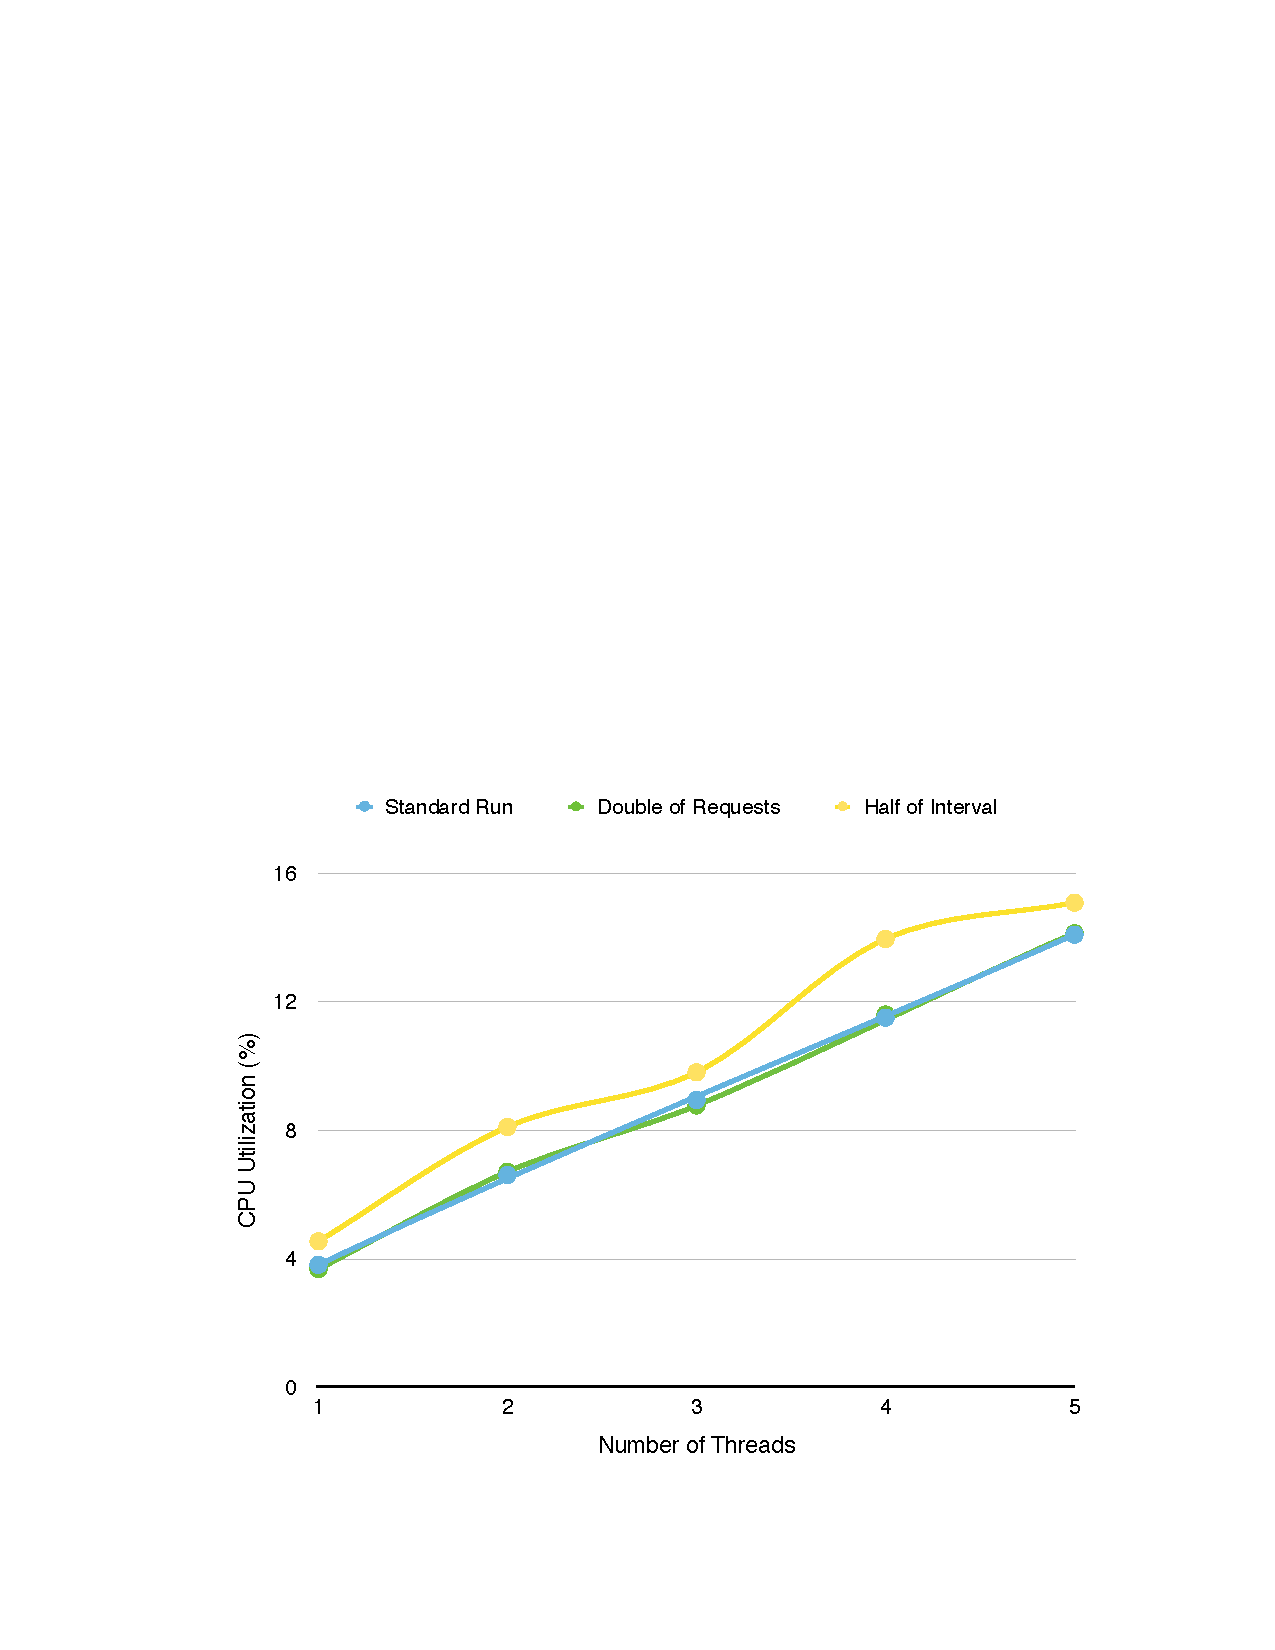
\includegraphics[width=\linewidth]{./images/cpu_1_lap}
  \caption{CPU Utilization performance results.}
  \label{fig:eval_baseline_cpu}
\end{subfigure}%
\begin{subfigure}{.5\textwidth}
  \centering
  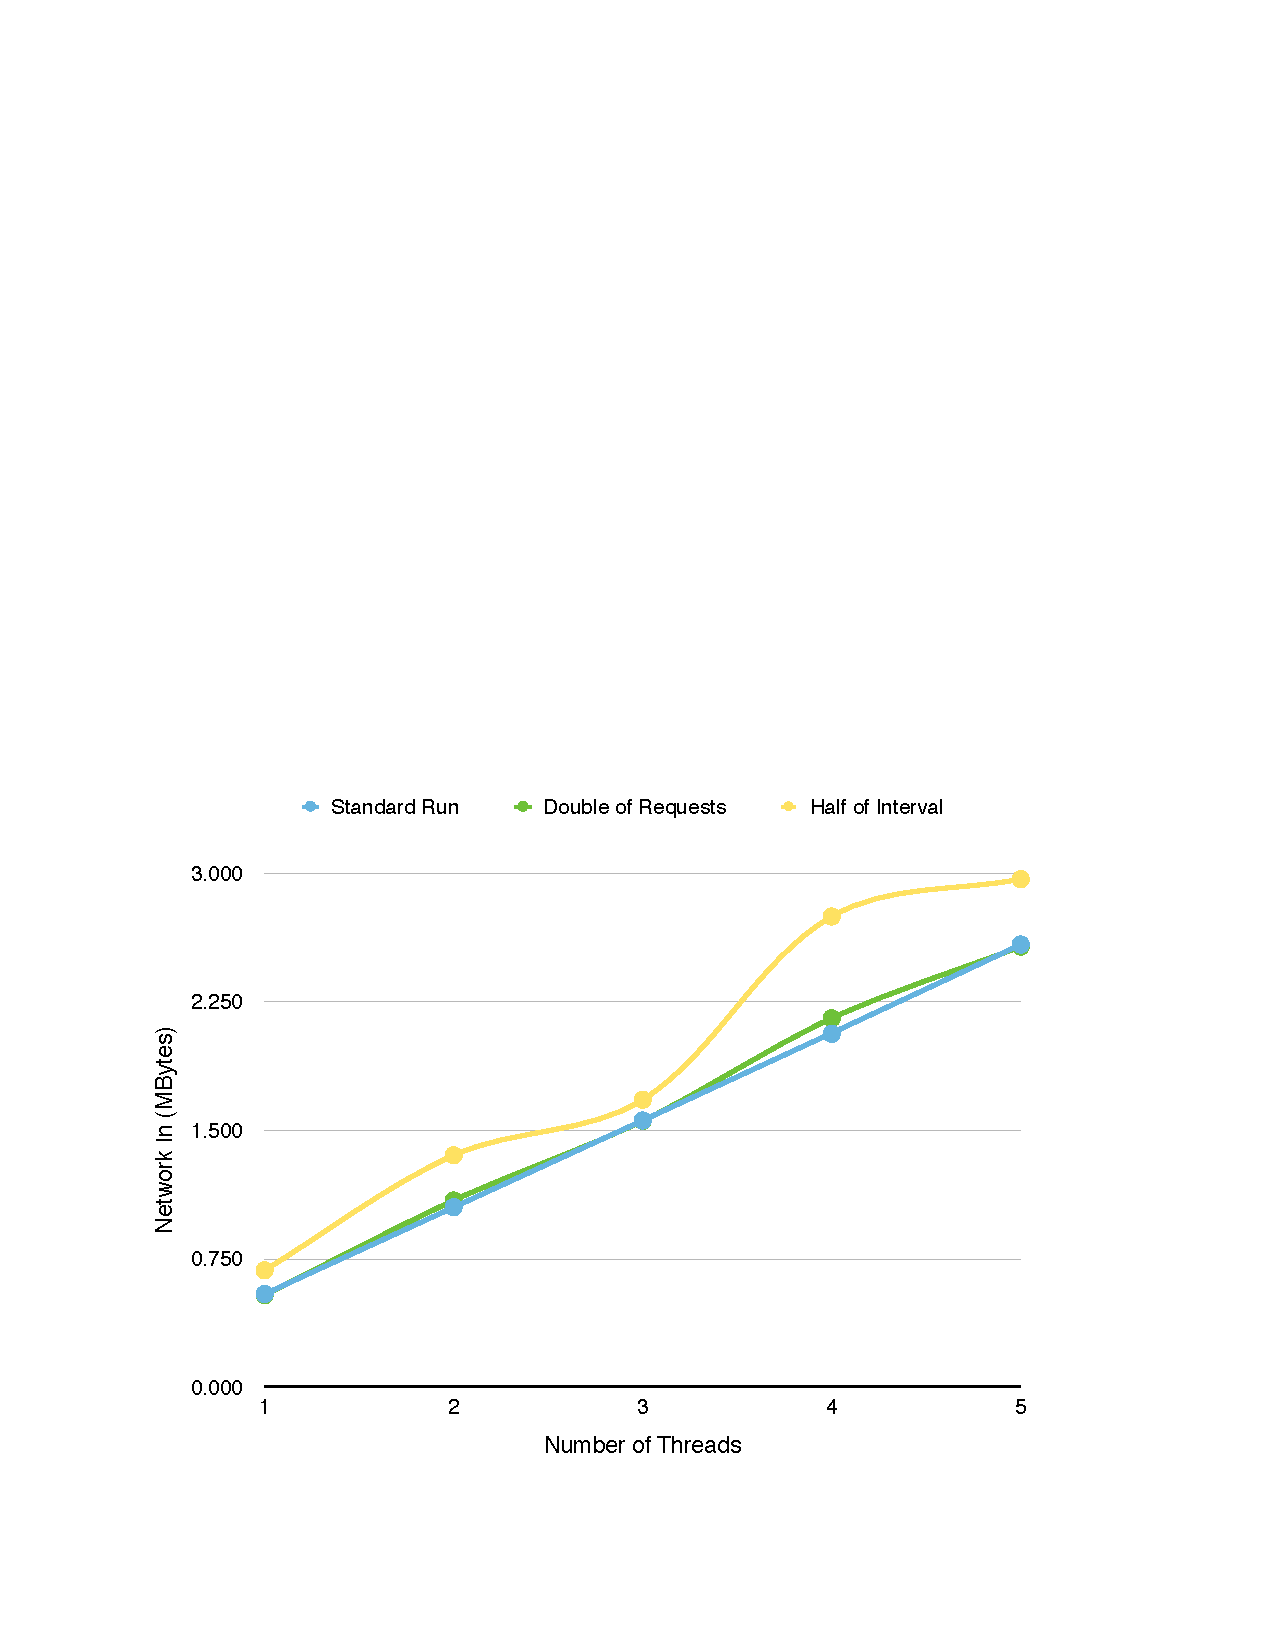
\includegraphics[width=\linewidth]{./images/network_1_lap}
  \caption{Network traffic performance.}
  \label{fig:eval_baseline_network}
\end{subfigure}
\caption[Data storage: Baseline results.]{Data storage performance: Baseline evaluation results.}
\label{fig:eval_baseline_results}
\end{figure}

Figure~\ref{fig:eval_baseline_cpu} presents the system metric \textit{CPU Utilization} for the current
experiment. Comparing the values obtained in the experiment for the proposed variations, the
\textit{Standard} and \textit{Double of Requests} variations the presents similar results -
maximum close to $\approx14\%$ - and its behavior tend to assume a linear pattern. For the \textit{Half of Interval}
variation, it is possible to observe that the metric value is always higher - maximum close to $\approx16\%$ -
when compared with the other variations. The metric behavior changes according the number of threads
that are sending events and tend to take a sinusoidal pattern.\\

The system metric \textit{Network In}, presented in Figure~\ref{fig:eval_baseline_network}, assumes a
similar behavior of the previous metric. For the \textit{Standard} and \textit{Double of Requests} variations,
they presented similar results - maximum close to $\approx2.5$ \gls{MB} - and its behavior tend to assume a linear
pattern. It is possible to take the same conclusions for the \textit{Half of Interval} variation,
where the results are always higher - maximum close to $\approx3$ \gls{MB} - and the behavior tends to assume
a sinusoidal pattern.

\subsubsection{Track 3 Laps}
\label{subs:eval_exp_data_3laps}
In this scenario the session contains the data recorded based in the events generated during 3 laps
in the track. The parameters used to execute the test for this scenario are described in
Table~\ref{tab:3laps_parameters}.\\

% 3 Lap parameters
\begin{table}[ht!]
  \begin{tabular}{|c|c|}
    \hline
    Number of Events & Period \\ \hline
    8895             & 57ms   \\ \hline
  \end{tabular}
  \caption[Data storage: 3 Lap evaluation parameters.]{Data storage performance: 3 Lap evaluation parameters.}
  \label{tab:3laps_parameters}
\end{table}

% 3 Lap results
\begin{figure}[ht!]
\centering
\begin{subfigure}{.5\textwidth}
  \centering
  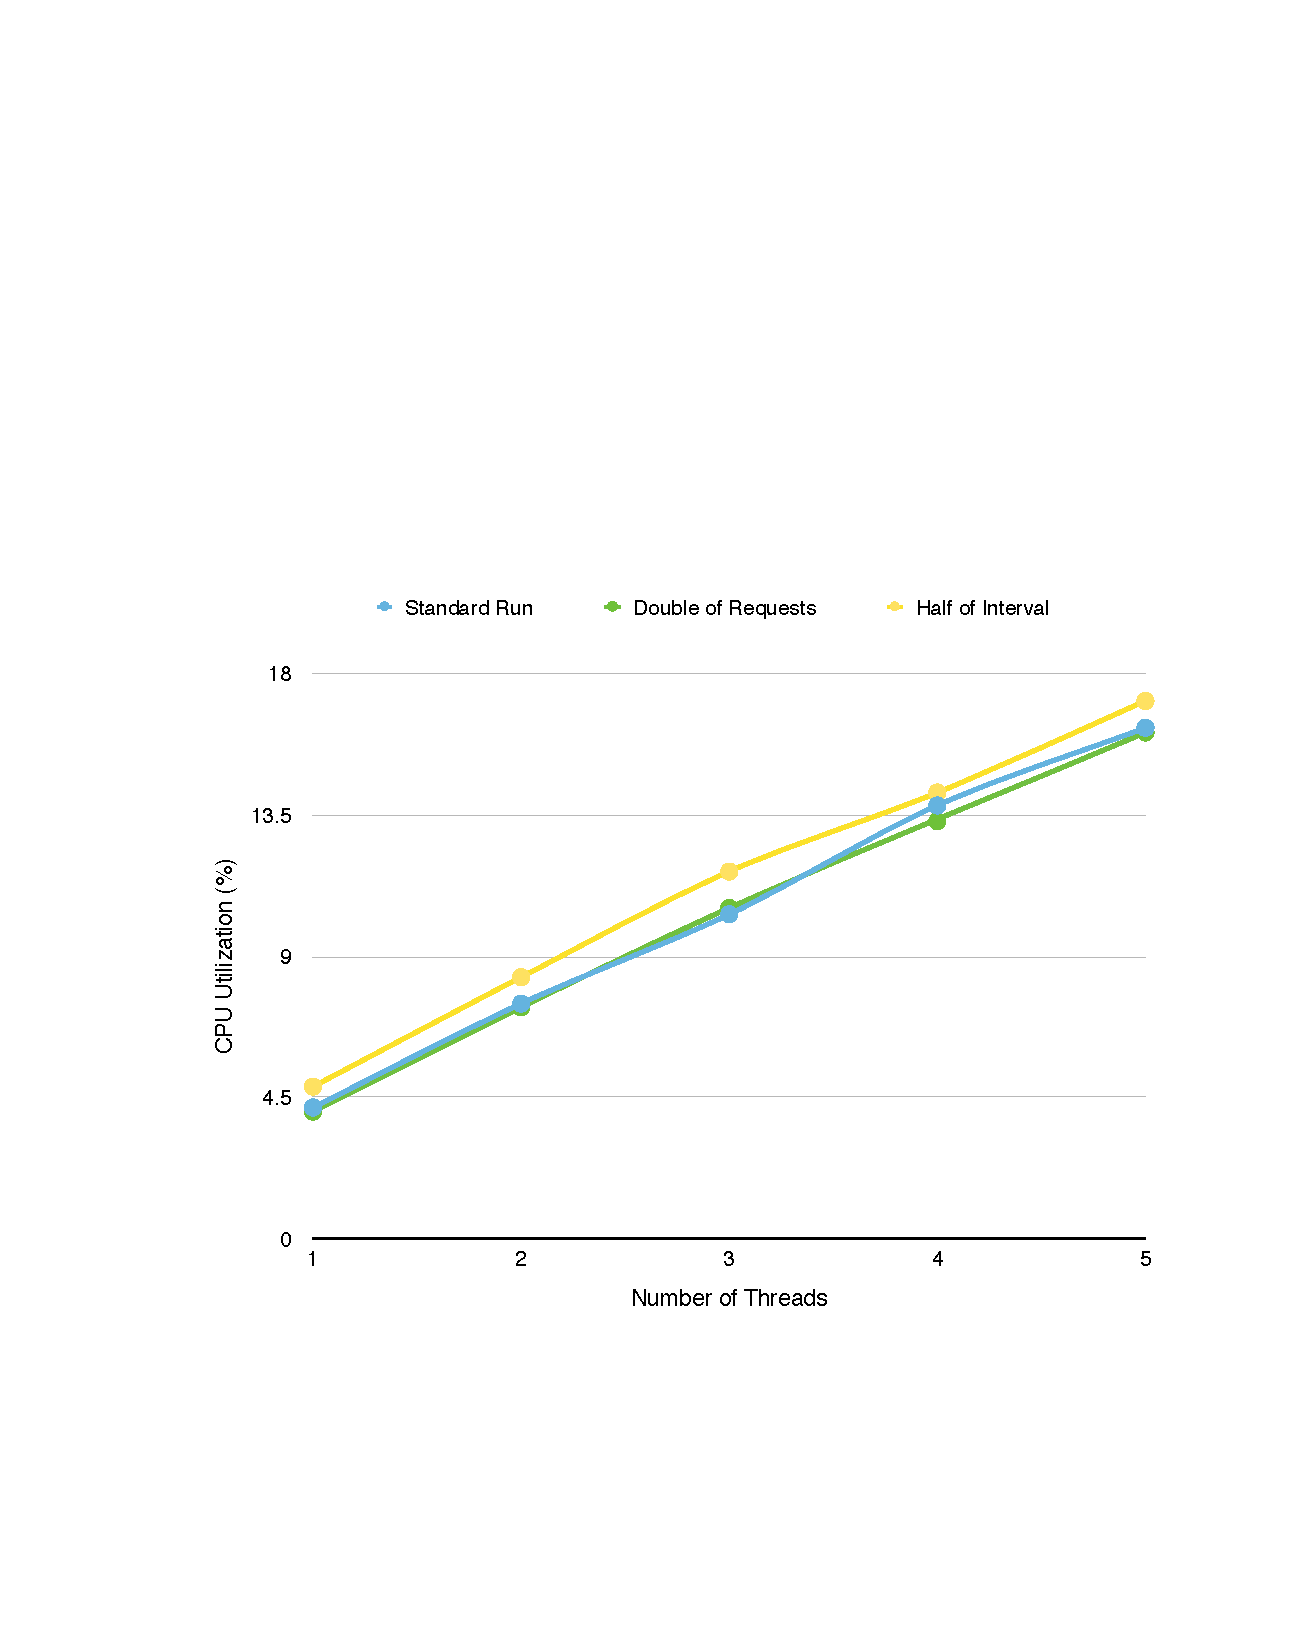
\includegraphics[width=\linewidth]{./images/cpu_3_lap}
  \caption{CPU Utilization performance results.}
  \label{fig:eval_3laps_cpu}
\end{subfigure}%
\begin{subfigure}{.5\textwidth}
  \centering
  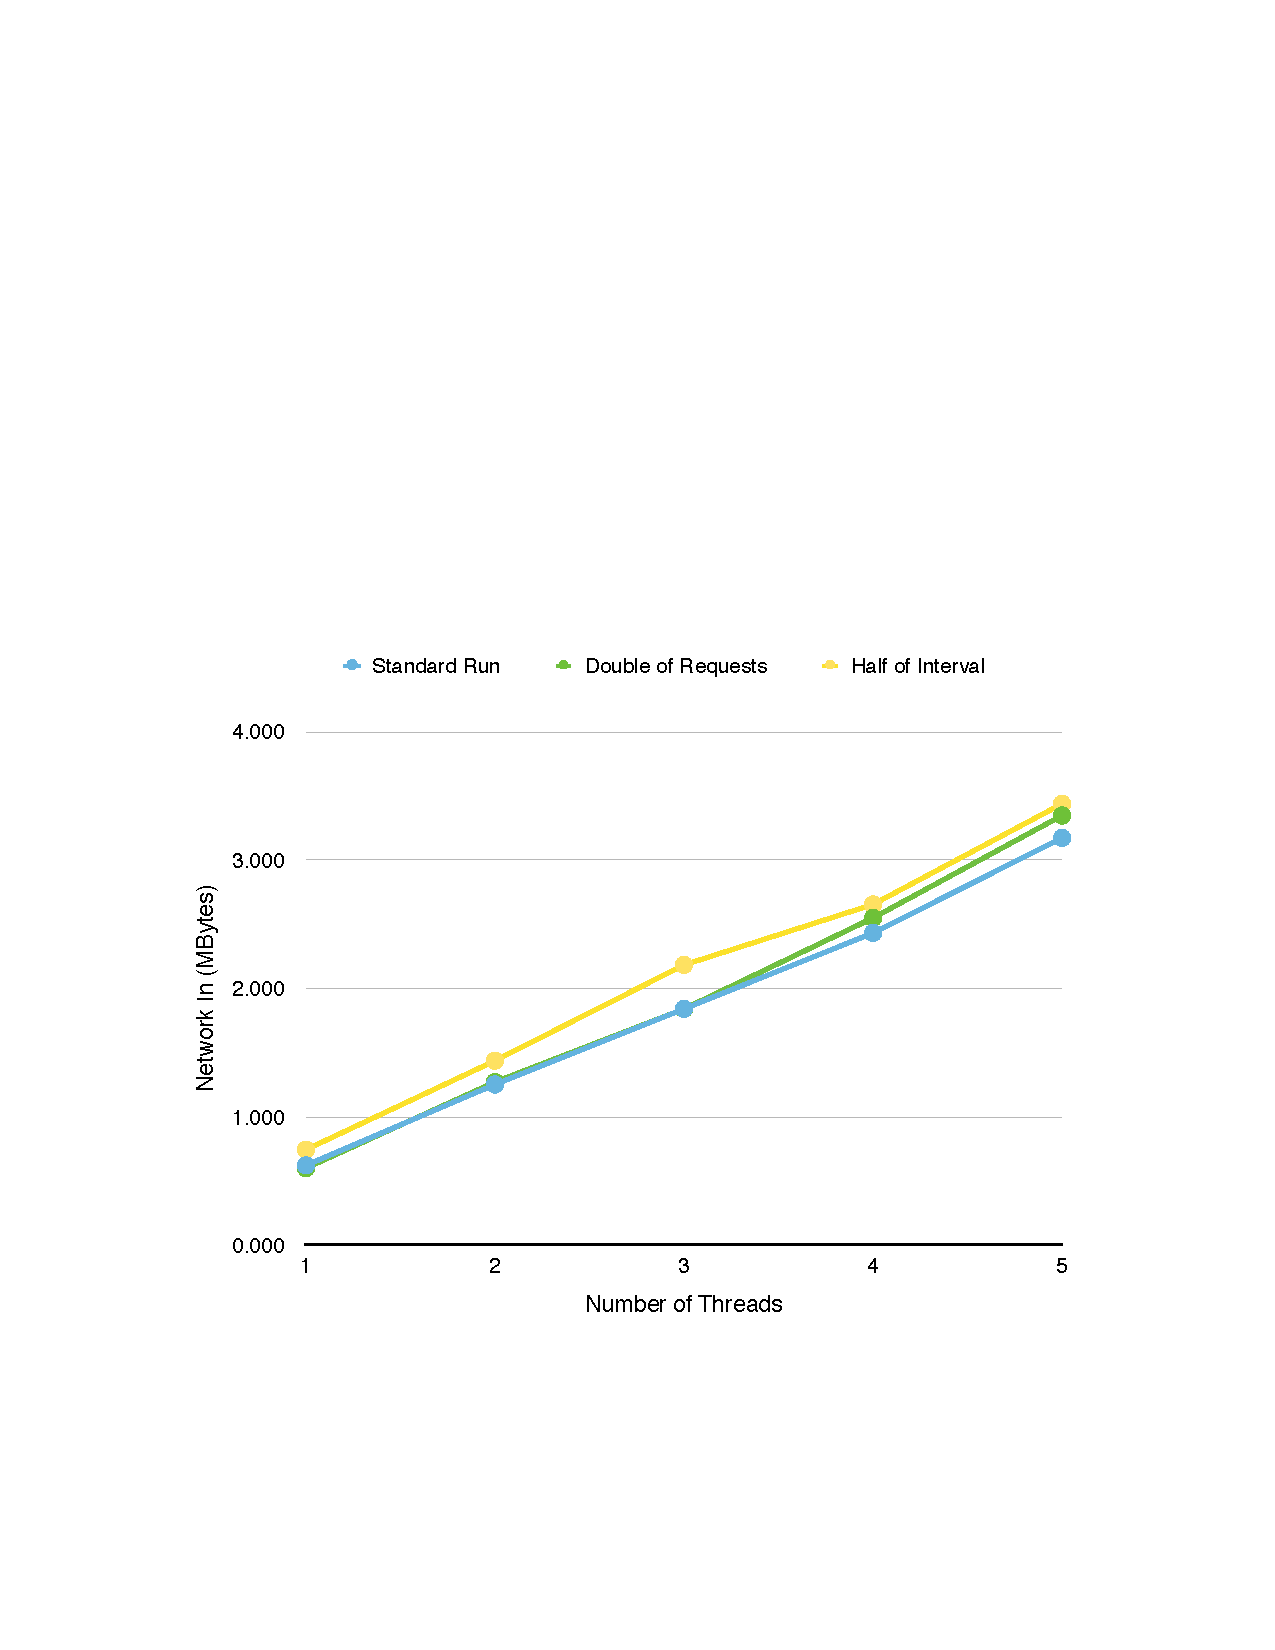
\includegraphics[width=\linewidth]{./images/network_3_lap}
  \caption{Network traffic performance results.}
  \label{fig:eval_3laps_network}
\end{subfigure}
\caption[Data storage: 3 Lap performance results.]{Data storage performance: 3 Lap performance results.}
\label{fig:eval_3laps_results}
\end{figure}

Figure~\ref{fig:eval_3laps_cpu} presents the system metric \textit{CPU Utilization} for the current
experiment. Comparing the results obtained in the experiment, it is possible to conclude that
they are very similar for all variations. The \textit{Half of Interval} continues to present
the highest values - maximum close to $\approx18\%$ - while the other variations presents almost identical
results - maximum close to $\approx16\%$. Regarding the metric behavior, all variations tends to assume
a linear pattern.\\

As in the previous experiment, the system metric \textit{Network In}, presented in Figure~\ref{fig:eval_3laps_network},
is very similar to the previous regarding its values and behavior. The \textit{Half of Interval}
variation still presents the highest values - maximum close to $\approx3.5$ \gls{MB} - but as the number of
threads increase, it is possible to observe that the values of the \textit{Double of Requests}
variation tend to be close to the \textit{Half of Interval}.

% Evaluation Analysis
\section{Results Analysis and Discussion}
\label{sec:eval_analysis}
Here we present the result analysis and discussion based on the results obtained in the performed
experiments.

% Latency Interaction
\subsubsection{Latency Interaction}
\label{subs:eval_results_latency}
Regarding the latency interaction, the results presented in Tables~\ref{table:fog_metrics} and
\ref{table:cloud_metrics} show that the fog-approach presented a better overall performance than
the cloud-based approach.

\subparagraph{Event Latency}
\label{subp:eval_event_latency}
Regarding the results for the \textit{Event Latency} metric, the fog-based approach presented the
best results. In order to meet the requirement \textit{R1}, the event latency must be less than
5s. According the results it is possible to conclude that both approaches meet \textit{R1}, but only
when the \gls{ALE} is configured with the \textit{Half-period ECspec}.

\subparagraph{Network Latency}
\label{subp:eval_network_latency}
The most relevant results are in network latency values for both approaches. The values for the \textit{Upload}
and \textit{Reponse} metrics presented a substantial difference, where the fog-based approach is the
best one. This allows to conclude that only the fog-approach is able to meet the requirement \textit{R2}.\\

However, it is important to point that there some aspects that can improve the network latency
of the cloud-based approach. For instance, the network connection is a possible bottleneck for the
performance of such approach. We believe that if the experiments were conducted through a faster
network connection - e.g. a Fiber-optic connection - the overall performance of the cloud-approach
will be better, but far from the fog-based approach.

\subparagraph{Idle Time}
\label{subp:eval_idle_time}
Another important concern regards with the \textit{ECspec} configuration. In the experiments
performed for both approaches, we notice that the time where the \gls{ALE} module remains in an idle
state decreased significantly when the defined \textit{ECspec} was configured with a smaller period.
However, in all experiments performed the \gls{ALE} spent more time in the idle state than
processing the events. Based on these results we are able to conclude that none of the approaches
meet the requirement \textit{R3}.

\subparagraph{Tag Data Processing}
\label{subp:eval_tag_processing}
During the evaluation process we noticed a behavior at the performance of the Fosstrak platform.
In the experiments performed for both fog-based and cloud-based approaches we observe that when
the \gls{ALE} module is configured with a \textit{Half-period ECspec}, it takes more time to
process the data from the \gls{RFID} tags. The reason for this performance behavior is unknown and
need more tests and further investigation in order to determine what causes that performance issue.

% Data Performance
\subsubsection{Data Storage Performance}
\label{subs:eval_results_data}
Regarding the data storage performance for the Fosstrak middleware, is possible to conclude that the metrics
of \textit{CPU Utilization} and \textit{Network In} increase as the threads and requests are growing.
These results are consistent with the ones obtained by Gomes et al. \cite{gomes2014future}, which
proposes a new \gls{IoT} infrastructure for \gls{EPC}Global middleware. Furthermore, in the experiments
performed Gomes detected that when the \textit{CPU Utilization} crosses the value of 95$\%$, the
outbound traffic started to decrease. After analyzing the stored data, the conclusion was that the
\gls{CPU} exhaustion caused by the \gls{EPCIS} affected the performance of \gls{ALE} module - when
executed in the same machine - resulting in a delay of data storage in the \gls{EPCIS} repository,
which explains the observed behavior.\\

According these results, is reasonable to assume that the performance of the data storage mechanism of
the Fosstrak implementation can be a bottleneck. However, in the general case the overall performance
is able to meet the requirements defined for our scenario (\textit{R4}).

\subsubsection{Cloud or Fog?}
\label{subs:eval_conclusion}
The obtained results show that a fog-based approach offers better overall performance to deploy a
smart warehouse application based in \gls{RFID} technology that requires low latency interaction.
But it will be this approach the best choice for all application domains?\\

Table \ref{table:smart_places_characteristics} summarizes the main characteristics of several
\gls{IoT} application domains. For instance, for application domains with a small network size, low network
bandwidth requirements, low scalability and that does not require low latency interaction - such as Ambient
Intelligence and Retail - a cloud-based approach is suitable, but probably the more adequate
solution it will be to provisioning the infrastructure in local, since that in most cases a local
server is able to host such applications.\\

For domains with a medium/large network size and network bandwidth requirements, that does not require
low latency interaction, but presents high scalability - such as Smart Agriculture and Smart Water
scenarios - a cloud-based approach is the most reasonable choice.\\

Finally, for domains with a medium/large network size and network bandwidth requirements, that requires
low latency interaction and presents high scalability - such as Smart Cities, Smart Transportation and
Healthcare - the fog-based approach is the best solution.
